\RequirePackage[2020-02-02]{latexrelease}


% Template for seminar reports
% Computer Vision Group, Visual Computing Institute, RWTH Aachen University
\documentclass[twoside,a4paper,article]{combine}
\usepackage[utf8]{inputenc}
\usepackage{a4}
\usepackage{fancyhdr}   
%\usepackage{german}    % Uncomment this iff you're writing the report in German
\usepackage{makeidx}
\usepackage{color}
\usepackage{t1enc}		% German letters in the "\hyphenation" - command
\usepackage{latexsym}	% math symbols
\usepackage{amssymb}    % AMS symbol fonts for LaTeX.
\usepackage{graphicx}
\usepackage{pslatex}
\usepackage{ifthen}
\usepackage{booktabs}
\usepackage[T1]{fontenc}
\usepackage{pslatex}
\usepackage{psfrag}
\usepackage{subfigure}
\usepackage{url}
\usepackage{datetime}
\usepackage{xspace}
\usepackage{newtxmath}

\usepackage{float}
\usepackage{subcaption}

\usepackage[table]{xcolor}% http://ctan.org/pkg/xcolor
\usepackage{listings}




\newdateformat{monthyeardate}{\monthname[\THEMONTH] \THEYEAR}

% Do not change these sizes and do not add superfluous 
% pagebreaks to increase the page count.
\setlength{\oddsidemargin}{3.6pt}
\setlength{\evensidemargin}{22.6pt}
\setlength{\textwidth}{426.8pt}
\setlength{\textheight}{654.4pt}
\setlength{\headsep}{18pt}
\setlength{\headheight}{15pt}
\setlength{\topmargin}{-41.7pt}
\setlength{\topskip}{10pt}
\setlength{\footskip}{42pt}
\setlength{\parindent}{0pt}

\makeatletter
\DeclareRobustCommand\onedot{\futurelet\@let@token\@onedot}
\def\@onedot{\ifx\@let@token.\else.\null\fi\xspace}
\def\eg{\emph{e.g}\onedot} \def\Eg{\emph{E.g}\onedot}
\def\ie{\emph{i.e}\onedot} \def\Ie{\emph{I.e}\onedot}
\def\cf{\emph{c.f}\onedot} \def\Cf{\emph{C.f}\onedot}
\def\etc{\emph{etc}\onedot} \def\vs{\emph{vs}\onedot}
\def\wrt{w.r.t\onedot} \def\dof{d.o.f\onedot}
\def\etal{\emph{et al}\onedot}
\makeatother

% =========================================================================
\graphicspath{{pictures/}}
\setcounter{secnumdepth}{3}
\setcounter{tocdepth}{3}

% =========================================================================
\begin{document}
% Template for seminar reports
% Seminar Current Topics in Computer Vision and Machine Learning


\begin{titlepage}
    \begin{center}
    \ 
    \vspace{3.5cm}
    
    \textsf{
    RWTH Aachen University \\
    Faculty of Mathematics, Computer Science and Natural Sciences\\
    Chair of Computer Science 13 (Computer Vision) \\
    Prof. Dr. Bastian Leibe
    }
    
    \rule{\linewidth}{1pt}
    
    \vspace{1.75cm}
    \LARGE
    \textbf{Seminar Report}
    
    \vspace{1.7cm}
    \huge
    Linear and Nonlinear Filters
    
    \vspace{3.0cm}
    \Large
    Alexander Skretting\\
    \large
    Matriculation Number: 445457

    \vspace{1.0cm}
    \Large
    Jose Rigel Soeryo Soebandoro\\
    \large
    Matriculation Number: 444345
    
    \vspace{0.5cm}
    \monthyeardate\today
    
    \vspace{1.05cm}
    \rule{\linewidth}{1pt}
    
    \vspace{0.5cm}
    \textsf{\textbf{
    \normalsize
    \begin{tabular}{ll}
    Advisor:  & George Lydakis\\
    \end{tabular}
    }}
    \end{center}
\end{titlepage}



\begin{abstract}
% +++++++++++++++++++++++++
% Insert your Abstract here (one paragraph summary)
% +++++++++++++++++++++++++
\end{abstract}

\tableofcontents
\newpage
% =========================================================================

\section{Introduction}
Every picture created is different, from the camera they are taken with, the color space, to the subjects on the picture itself. As humans, we have trained our eyes to adjust our perceptions to
understand the pictures better and take information as we need through the context gathered from day to day life. This is unfortunately not the case for computers. Varying qualites and scenarios makes it
hard for computers to handle images and extract necessary informations.

This is where filtering is utilized to pass through and create a desired output image, catering to one' individual goals. The two major categories of filtering in Image processing are \emph{Linear} and \emph{Nonlinear filters}, with each
having variations of their own, tailored to their specific use cases, whether for noise suppresion, edge detection or image enhancement\cite{MISRA2020289}. Not only are filters used in isolation, but they can aid
in further methods and algorithms in image processing, as they create aim to create clean and workable images for computers. The comparison between each filter is not only determining which filters produces the highest quality output, yet
also defined by its computing complexity, both in space and time complexity. Optimizing these filters by means of different algorithms and strategies while maintaining its quality is highly preferable.

The two major categories of filtering in image processing are \textbf{\emph{Linear Filters}} and \textbf{\emph{Non-linear Filters}}. Linear Filtering is a simpler, yet powerful strategy for image processing, as they
only require a linear neighborhood operation to calculate the output image. For difficult scenarios however, it may not be possible to only rely on basic multiplications and sums. This is where Non-linear filters comes in handy, as they
feature concepts such as cellular automata. This article aims to discuss different types of filters, their applications and how each of them provides different benefits\footnotemark\footnotetext{Written by Jose}
\section{Linear Filters}
With \textbf{Linear Filtering}, or specifically linear spatial filtering, the function which is used to pass the image through
must be linear and shift invariant. The function $\pmb{L}$ is considered linear if there exists two constants $a$ and $b$ for any
two input pixels $f_1(m, n)$ and $f_2(m, n)$ such that

\begin{align*}
    \implies & g_1(m, n) = \boldsymbol{L} [f_1(m, n)] \land g_2(m, n) = \boldsymbol{L} [f_2(m, n)] \\
    \implies & a \cdot g_1(m, n) + b \cdot g_2(m, n) = \boldsymbol{L} [a \cdot f_1(m, n) + b \cdot f_2(m, n)]
\end{align*}

also called the \emph{superposition property of linear systems}\cite{BovikActon09}. Whereas a function is considered \emph{shift invariant} when
\begin{align*}
    \implies & g(m, n) = \boldsymbol{L} [f(m, n)]\\
    \implies & g(m - p, n - q) =  \boldsymbol{L} [f(m - p, n - q)]
\end{align*} $p$ and $q$ implies a spatial shift to both the input and output pixels\cite{BovikActon09}. An intuitive way to think
of these two properties is that the function has to behave the same throughout the entire picture.

\subsection{Correlation and Convolution Filtering}
A common formula for linear filtering is the \emph{Correlation Filtering}\cite{BovikActon09}. 
\[
    g(i,j) = \sum_{l \in \mathscr{M}}\sum_{k \in \mathscr{N}}{f(i+k, j+l) \cdot h(k, l)}
\]
or commonly notated as $g = f \otimes h$.

The desired output pixel $g(i, j)$, where $i$ and $j$ specify the
coordinates of it, is based on a $M \times N$ sized neighborhood, 
meaning not only does one pixel define an output pixel, but also a specified number
of its neighbors. The influence of each pixel in the neighborhood is defined by the filter coefficient $h(k, l)$,
also called its \emph{kernel} or \emph{mask}\cite{Szeliski_2022}. With this formula, it is possible to have a kernel that is rectangular and not square,
but through convention, it is generally preferred to have the kernel be square. As later discussed, square matrices are also more cost effective to calculate.

\[
\underbrace{
    \begin{bmatrix}
        128 & 34 & 123\\
        68 & 54 & 73 \\
        100 & 95 & 17
    \end{bmatrix}}_{\text{input neighborhood}}
\otimes
\underbrace{
    \begin{bmatrix}
        0.1 & 0.1 & 0.1\\
        0.1 & 0.2 & 0.1\\
        0.1 & 0.1 & 0.1
    \end{bmatrix}}_{\text{kernel}}
= 75
\]

As the above example with a $3 \times 3$ kernel, a total of 9 pixels is needed to calculate a single output pixel.

Another common variant on the formula is having the signs of the offsets reversed. 
\[
    g = f \ast h
\]
\[
    g(i,j) = \sum_{l \in \mathscr{M}}\sum_{k \in \mathscr{N}}{f(i-k, j-l) \cdot h(k, l)}
\]
With this formula, $\ast$ is called the \emph{convolutional} operator, and the kernel $h$ is called the \emph{impulse response function}. 
An interesting note is that, when the kernel $h$ is convolved with an impulse signal $\delta$ (an image with 0 everywhere except the origin),
it reproduces the kernel itself $h \ast \delta = h$, whereas with correlational filtering, 
it produces the reflected signal (inverted signal in both dimensions).\cite{Szeliski_2022} In cases
where the kernel is symmetrical on both axis (e.g. box blur), the result of convolutional and correlational is the same.

\begin{minipage}{\textwidth}\begin{figure}[H]
    \centering
    \subfigure[correlation]{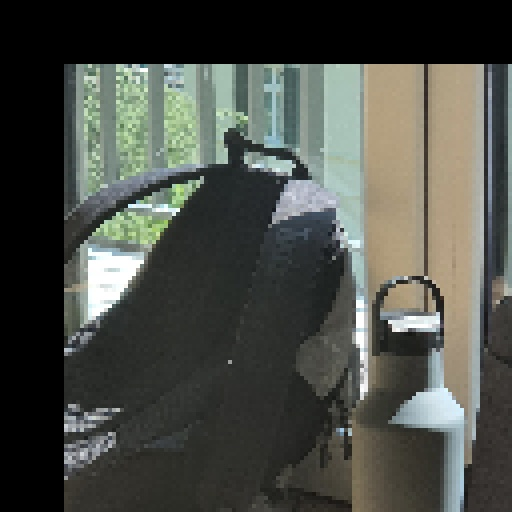
\includegraphics[width=0.19\textwidth]{img/correlation.jpg}}
    \subfigure[convolution]{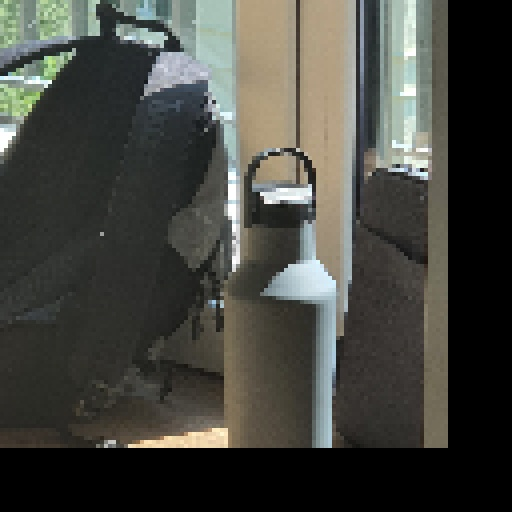
\includegraphics[width=0.19\textwidth]{img/convolved}}
    \caption{Difference between Correlation and Convolution Filtering by translating 32 pixels}
\end{figure}\end{minipage}

By rotating the kernel $180^\circ$, it is possible to get the same output from convolution filtering with correlational filtering and vice versa\cite{Gonzalez_Woods_2018}.

An apparent problem from neighborhood filtering is that on the edges, the neighbors simply does not exist in one or two directions 
(e.g. a $1000\times1000$ image passed through a $3\times3$ kernel would produce a $998\times998$ image). 
There are a couple method to alleviate the calculation of the nonexistent neighbors.

\subsection{Padding (Border Effects)}

\begin{minipage}{\textwidth}\begin{figure}[H]
    \centering
    \subfigure[zero]{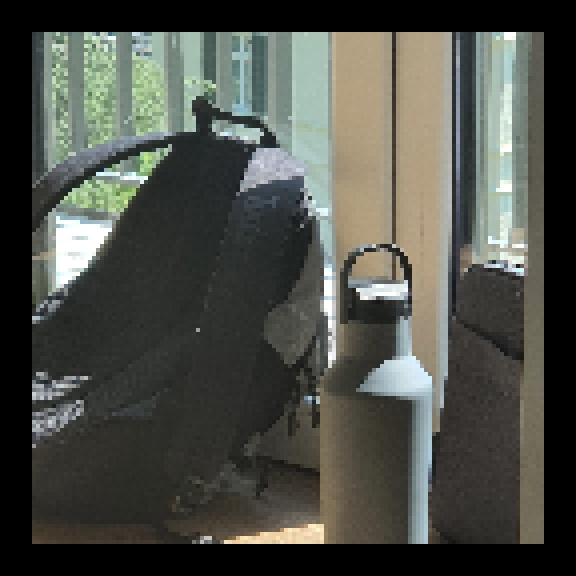
\includegraphics[width=0.19\textwidth]{img/border_constant}}
    \subfigure[wrap]{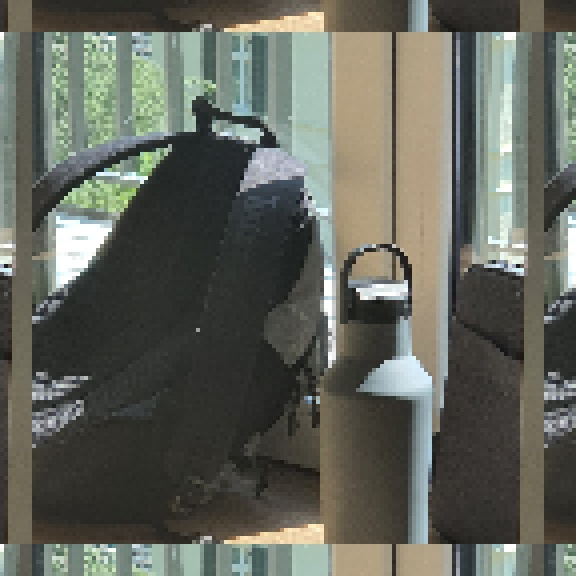
\includegraphics[width=0.19\textwidth]{img/border_wrap}}
    \subfigure[clamp]{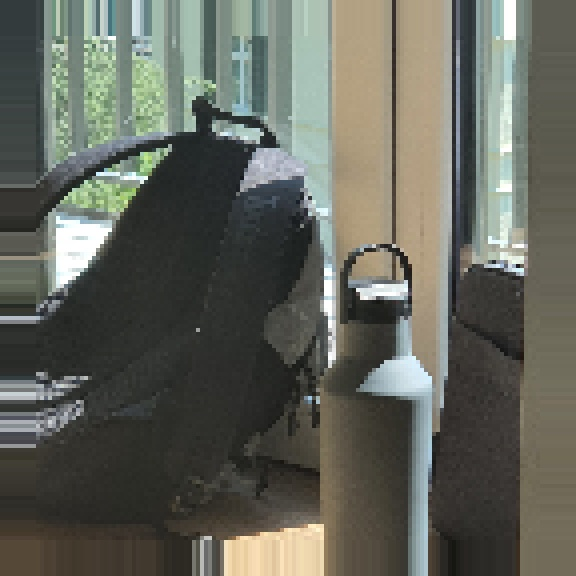
\includegraphics[width=0.19\textwidth]{img/border_clamp}}
    \subfigure[mirror]{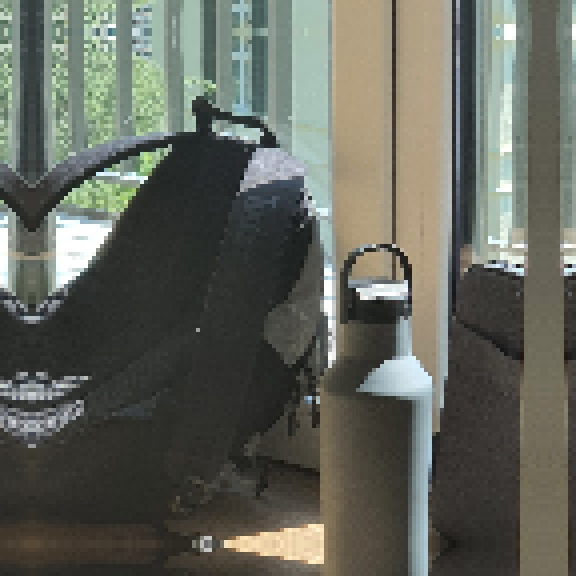
\includegraphics[width=0.19\textwidth]{img/border_reflect}}
    \subfigure[extend]{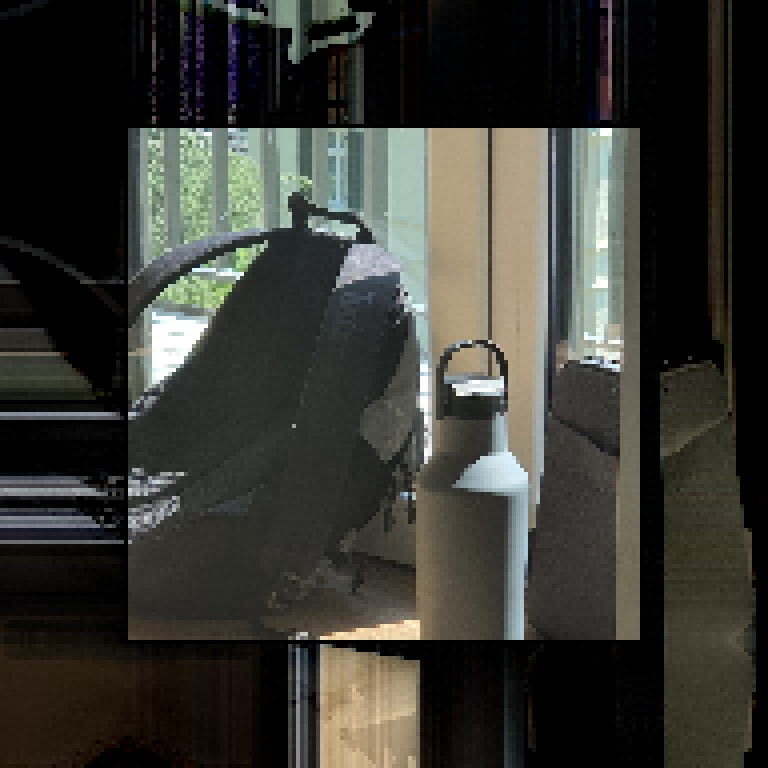
\includegraphics[width=0.19\textwidth]{img/border_extend.jpg}}
    \caption{Different types of border padding}
    \label{fig:padding_borders}
\end{figure}\end{minipage}
\begin{itemize}
    \item \textbf{Zero:} Set all pixels outside the region to zero.
    \item \textbf{Constant:} This is similar to Zero, but instead a specific color is chosen to replace the out of bound pixels.
    \item \textbf{Clamp:} The edge pixels are repeated indefinitely.
    \item \textbf{(Cyclic) Wrap (Repeat or Tile):} The entire image is repeated similar to tiling it infinitely.
    \item \textbf{Mirror:} The image is mirrored accordingly on each of the edges.
    \item \textbf{Extend:} This is a combination of clamping and mirroring, where the clamped image is subtracted with the mirrored image.
\end{itemize}\label{chap:padding}

This of course not only affects the unseen pixels, but the effects can bleed into the pixels inside the frame.
\begin{minipage}{\textwidth}\begin{figure}[H]
    \centering
    \subfigure[zero]{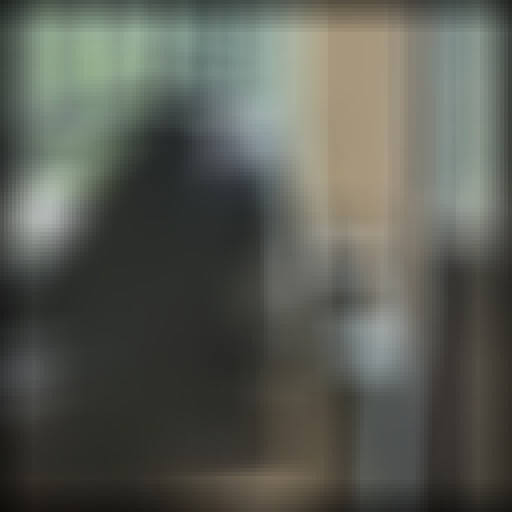
\includegraphics[width=0.19\textwidth]{img/boxBlur_constant}}
    \subfigure[wrap]{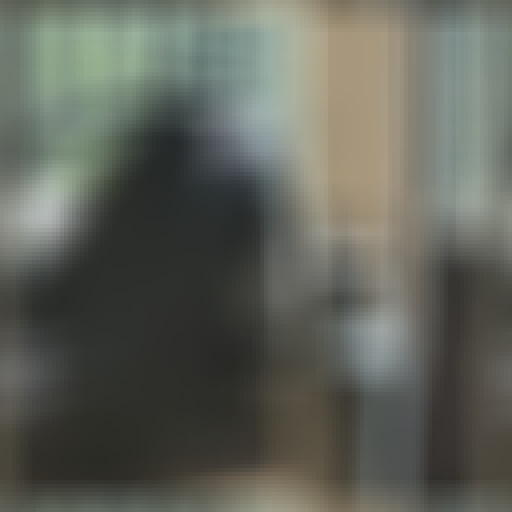
\includegraphics[width=0.19\textwidth]{img/boxBlur_wrap}}
    \subfigure[clamp]{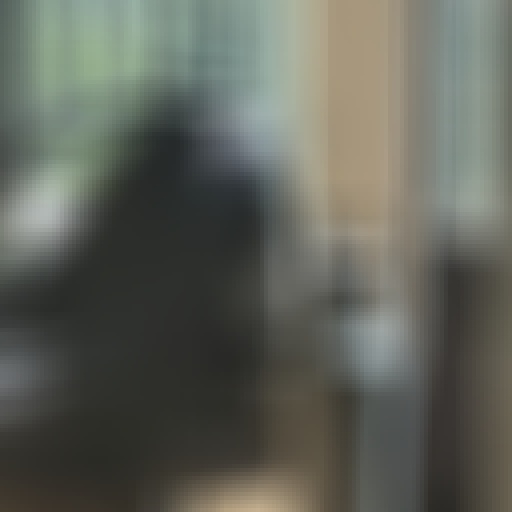
\includegraphics[width=0.19\textwidth]{img/boxBlur_clamp}}
    \subfigure[mirror]{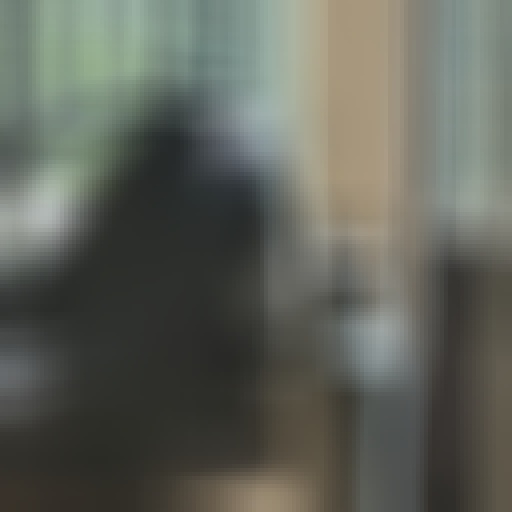
\includegraphics[width=0.19\textwidth]{img/boxBlur_reflect}}
    \subfigure[extend]{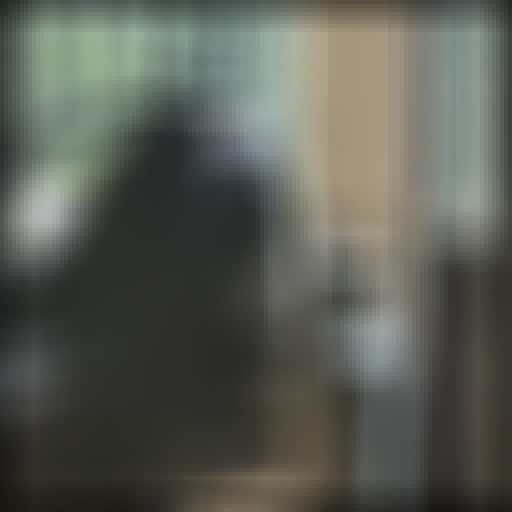
\includegraphics[width=0.19\textwidth]{img/boxBlur_extend.jpg}}
    \caption{Effects of different paddings with box blur}
    \label{fig:boxBlur_borders}
\end{figure}\end{minipage}

As seen from Figure \ref{fig:boxBlur_borders}, with a constant padding, the color chosen for the constant value bleeds uniformly in the edges. The wrapped image
can be convincing at times, but drastic changes from one border to another may lead to undesirable bleeding edges. If we instead clamp the image, the repeated pixels are noticeably
present, depending on the kernel size, this may still be desireable. In this use case, mirror seems to be the most convincing. It cannot however be said, that mirror is objectively the better
method, as it depends on the scenarios and use cases (e.g. if a subject is placed in a white background, then the constant padding may be desirable).

There are other ways to handle the borders such as two-phase duplication,
which is similar to clamp but alternates between the last 2 pixels.
A change in the filter function per individual basis can also be implemented, but it might not be practical,
as large amounts of additional logic may be needed\cite{BaileyAmbikumar18}.

\subsection{Separable Filtering}
The time complexity to calculate a single pixel can be said to be $O(M \cdot N)$ as it is dependent
on the size of the kernel. For each of the pixel in the kernel, it must be both multiplied and summed together
with its neighbors. This can be in practice sped up by separating the horizontal and vertical operations, hence performing
a one dimensional convolution horizontally, then one additional operation for the vertical convolution. This kernel in this case is the
outer product of two one dimensional kernels\cite{Szeliski_2022}. 
\[
    \boldsymbol{K} = v \otimes h = 
    \begin{bmatrix}
        v_1h_1 & v_1h_2 & v_1 h_3 & \hdots & v_1h_n \\
        v_2h_1 & v_2h_2 & v_2 h_3 & \hdots & v_2h_n \\
        \vdots & \vdots & \vdots & \ddots & \vdots \\
        v_m h_1 & v_m h_2 & v_m h_3 & \hdots & v_m h_n \\
    \end{bmatrix}
\]

Also notated as $K=vh^{\boldsymbol{T}}$, where $\boldsymbol{T}$ denotes transposing $h$, since both are supposedly vertical tuples.

A method to check whether a given Kernel is separable is to use \emph{Singular Value Decomposition (SVD)} \cite{Szeliski_2022}

\[        
    \boldsymbol{K} = \sum_{i}{\sigma_i \cdot u_i \cdot v_i^{\boldsymbol{T}}} 
\]
or more generally
\begin{align*}
        \boldsymbol{K} =& \textbf{U}_{m\times p} \boldsymbol{\textstyle\sum}_{p\times p} \textbf{V}_{p\times n}^{\boldsymbol{T}} \\
        \boldsymbol{K} =& \begin{bmatrix}
            u_0 & \hdots & u_{p-1}
        \end{bmatrix}
        \begin{bmatrix}
            \sigma_0&&\\
            &\ddots&\\
            &&\sigma_{p-1}
        \end{bmatrix}
        \begin{bmatrix}
            v_0 \\
            \vdots \\
            v_{p-1}
        \end{bmatrix}
\end{align*}
Note that it requires the number of rows and columns must be the same, it can however be solved by putting 0 as the missing rows/columns,
to allow the kernel to be a square matrix.Then the first singular value $\sigma_0$ is checked. If it is the only one that is non zero,
and the rest is zero, then the kernel is separable. As an example, the sobel filter, which is used for edge detection, 
can be separated into two separate operations. In this case, this is for the horizontal derivative approximation. \cite{CHANG2023160}
\[
    \frac{1}{8}
    \begin{bmatrix}
        -1 & 0 & 1 \\
        -2 & 0 & 2 \\
        -1 & 0 & 1
    \end{bmatrix}
    =
    \frac{1}{8}
    \begin{bmatrix} -1 & 0 & 1 \end{bmatrix}
    \begin{bmatrix} 1 \\ 2 \\ 1 \end{bmatrix}
\]
The normalization of the operators are easily calculated by dividing each operator with the absolute sum of the entries.
\[  
    \begin{bmatrix} -1 & 0 & 1 \end{bmatrix} \Rightarrow \vert -1 \vert + \vert 0 \vert + \vert 1 \vert = 2 \Rightarrow \frac{1}{2}
\]
Then the normalized operator is
\[
    \frac{1}{2} \begin{bmatrix} -1 & 0 & 1 \end{bmatrix}
\]
it applies to the vertical operator as well
\[
    \frac{1}{4} \begin{bmatrix} 1 \\ 2 \\ 1 \end{bmatrix}
\]
The following are more examples of common separable filtering.

\begin{center}\begin{tabular}{c c c c c}
    $
        \frac{1}{K^2}
        \begin{bmatrix}
           1 & 1 & \hdots & 1 \\
           1 & 1 & \hdots & 1 \\
           \vdots & \vdots & \ddots & \vdots \\
           1 & 1 & \hdots & 1
        \end{bmatrix}
    $
&
    $
        \frac{1}{16}
        \begin{bmatrix}
            1 & 2 & 1 \\
            2 & 4 & 2 \\
            1 & 2 & 1
        \end{bmatrix}
    $
& 
    $
        \frac{1}{256}
        \begin{bmatrix}
            1 & 4 & 6 & 4 & 1 \\
            4 & 16 & 24 & 16  & 4 \\
            6 & 24 & 36 & 24 & 6 \\
            4 & 16 & 24 & 16  & 4 \\
            1 & 4 & 6 & 4 & 1
        \end{bmatrix}
    $
& 
    $
        \frac{1}{8}
        \begin{bmatrix}
            -1 & 0 & 1 \\
            -2 & 0 & 2 \\
            -1 & 0 & 1
        \end{bmatrix}
    $
& 
    $
        \frac{1}{4}
        \begin{bmatrix}
            1 & -2 & 1 \\
            -2 & 4 & -2  \\
            1 & -2 & 1
        \end{bmatrix}
    $
\\
    $
        \frac{1}{K} 
        \begin{bmatrix} 1 & 1 & \hdots & 1 \end{bmatrix}
    $
&
    $
        \frac{1}{4} 
        \begin{bmatrix} 1 & 2 & 1 \end{bmatrix}
    $
&   
    $
        \frac{1}{16}
        \begin{bmatrix} 1 & 4 & 6 & 4 & 1 \end{bmatrix}
    $
&   
    $
        \frac{1}{2} 
        \begin{bmatrix} -1 & 0 & 1 \end{bmatrix}
    $
&
    $
        \frac{1}{2} 
        \begin{bmatrix} -1 & 2 & 1 \end{bmatrix}
    $
\\
Box & Bilinear & Gaussian & Sobel & Corner 
\end{tabular}\end{center}

Note that for Corner filtering, the kernel is not normalized. Normalization is important as otherwise, a pixel may go beyond the allowed value range.
In cases where the kernel has a negative value, it means that the pixel value is inverted, since an integer overflow occurs (e.g. $64
(-1)= -64 \mod 256 = 192$ for one channel in an 8 bit pixel).`'
With some filters, it is not always possible to separate it into just two operations, therefore it can be
transformed into a series of 1 dimensional operations. However, this may be impractical as it increases the time and space
complexity.

\subsection{Examples of Linear Filters}
Due to the fact that linear filter in essence is the sum of pixels in a neighborhood with varying weights and sizes, there are infinitely many different kernels that can
define operators which classified as linear and invariant. It is also even possible to factor in different color channels. As an example, it is possible to shift the hue of an image.
In this example, using a kernel of $\begin{bmatrix}0 & 0 & 1\end{bmatrix}$, the hue is shifted to the left (negative).
\lstset{language=Python}
\begin{lstlisting}
img = cv.imread("color.jpg")
kernel = np.array([[[0, 0, 1]]])
convolved = ndimage.convolve(img, kernel, mode='reflect')
cv.imwrite('../img/colorShift.jpg', convolved)
\end{lstlisting}


\begin{minipage}{\textwidth}\begin{figure}[H]
    \centering
    \subfigure[original]{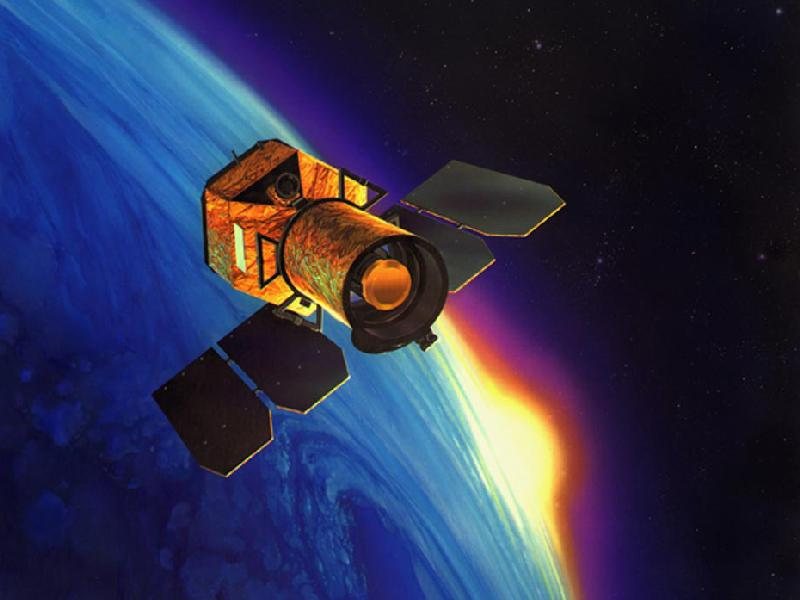
\includegraphics[width=0.30\textwidth]{codes/color.jpg}}
    \subfigure[shifted]{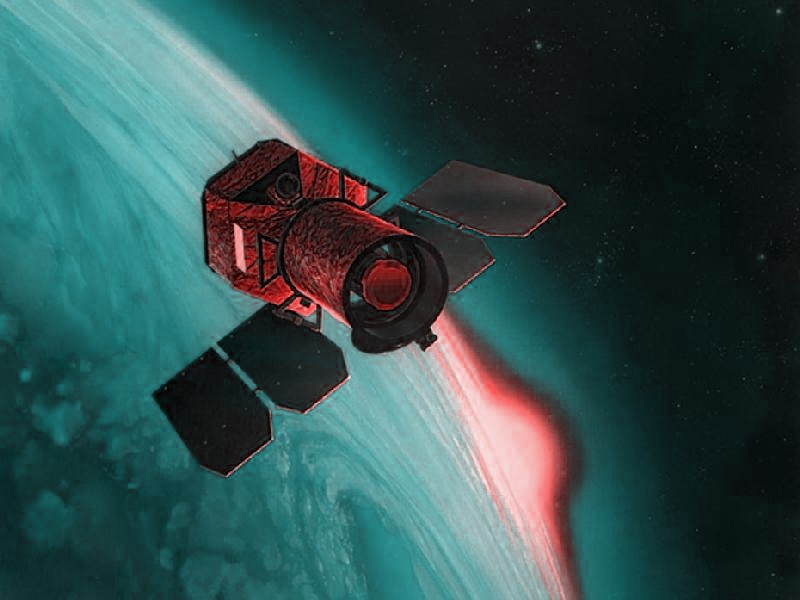
\includegraphics[width=0.30\textwidth]{img/colorShift.jpg}}
    \caption{Hue shifting using linear filters of the GALEX telescope image\cite{NASA_on_The_Commons_23}}
    \label{fig:hueshift}
\end{figure}\end{minipage}

The simplest application for linear filters are for smoothing(blurring) images. This not only serves their inherent purpose, but as later discussed, it can be used to aid other applications such as
edge detection or image enhancement.
\begin{itemize}
    \item \textbf{Box Filter:} each pixel is determined by the average of a $K \times K$ 
        neighborhood of pixels. It is also often called the \emph{moving average}, as the calculation can be done with scanlines, subtracting the
        old pixel and adding the newest pixels to the running sum. As the pixel is influenced equally by a square neighborhood, this may not be ideal as some `square artifacts' can be seen.
    \item \textbf{Bartlett Filter:} one solution to this is by separably convolving the image
        with a linear `tent' function (having its peak in the middle). A $3\times 3$ version of this is called the bilinear kernel.
    \item \textbf{Approximate Gaussian Filter:} if the Bartlett kernel is convolved with itself, this will produce an approximate version of the gaussian kernel.
\end{itemize}

This intuitively can be used to reduce the amount of noise on a picture. However, since it naively blurs the entire image,
details are also lost in the process.\\
\begin{minipage}{\textwidth}\begin{figure}[H]
    \centering
    \subfigure[original]{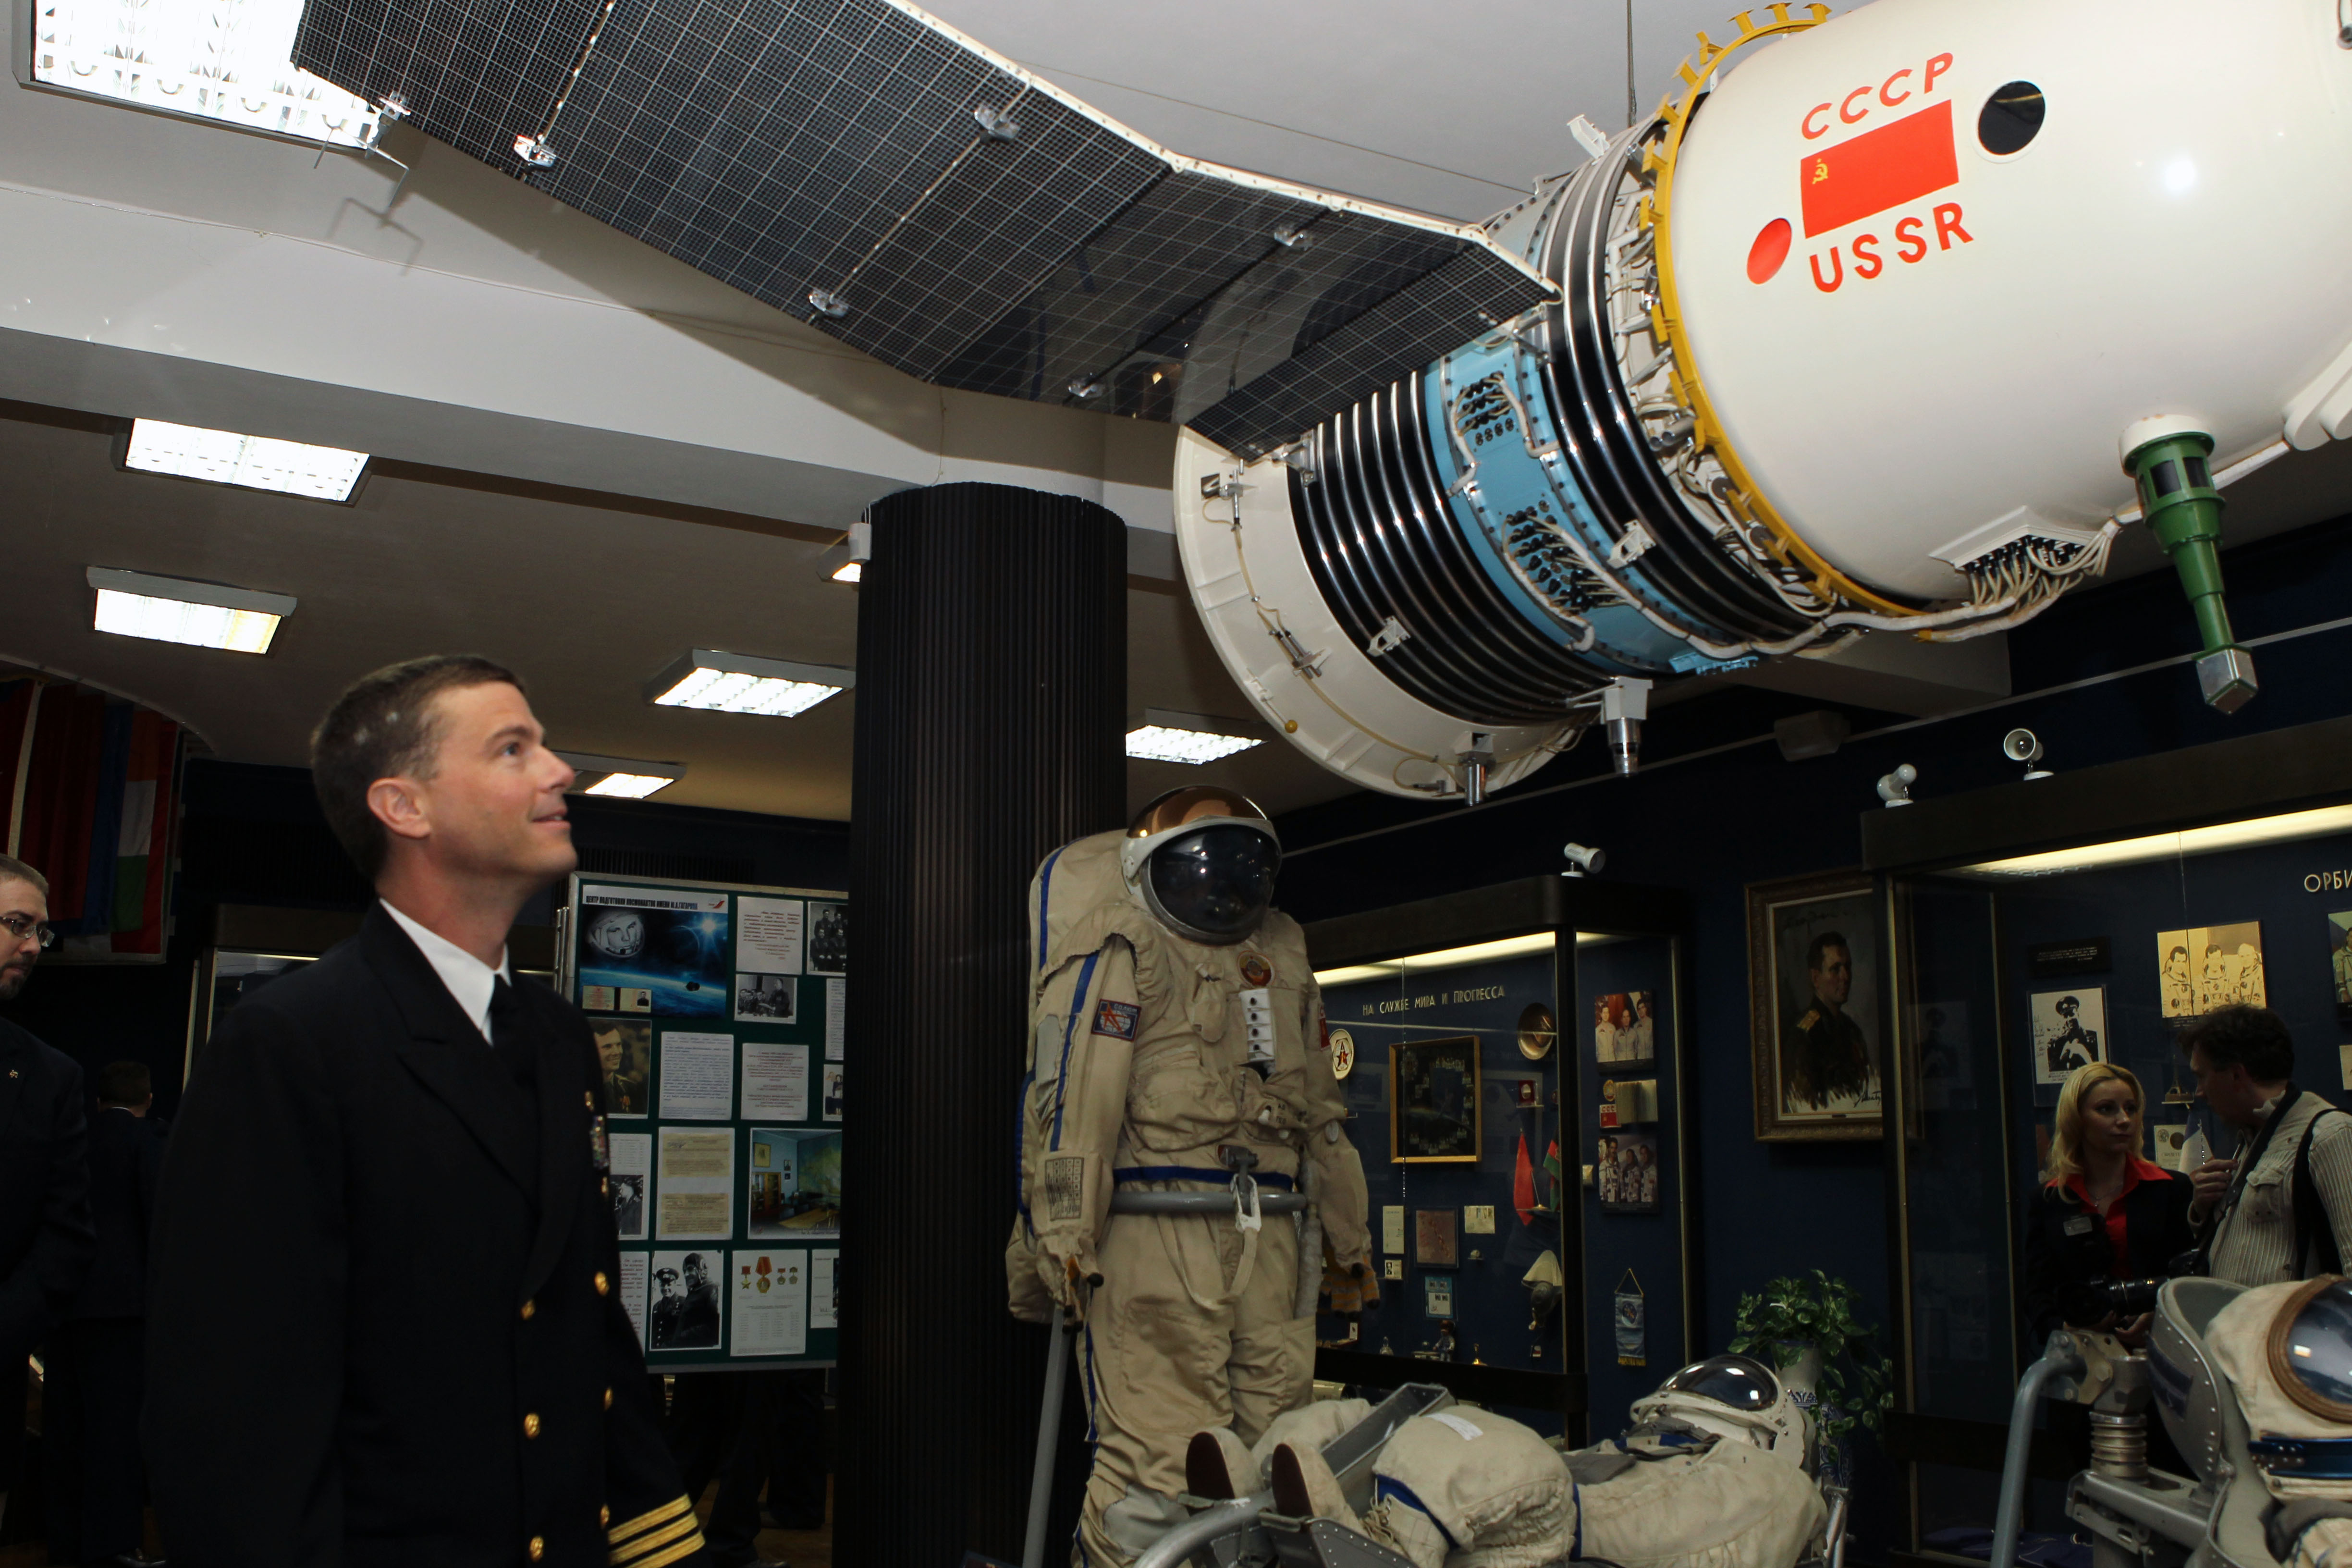
\includegraphics[width=0.32\textwidth]{codes/original_noise.jpg}}
    \subfigure[noise]{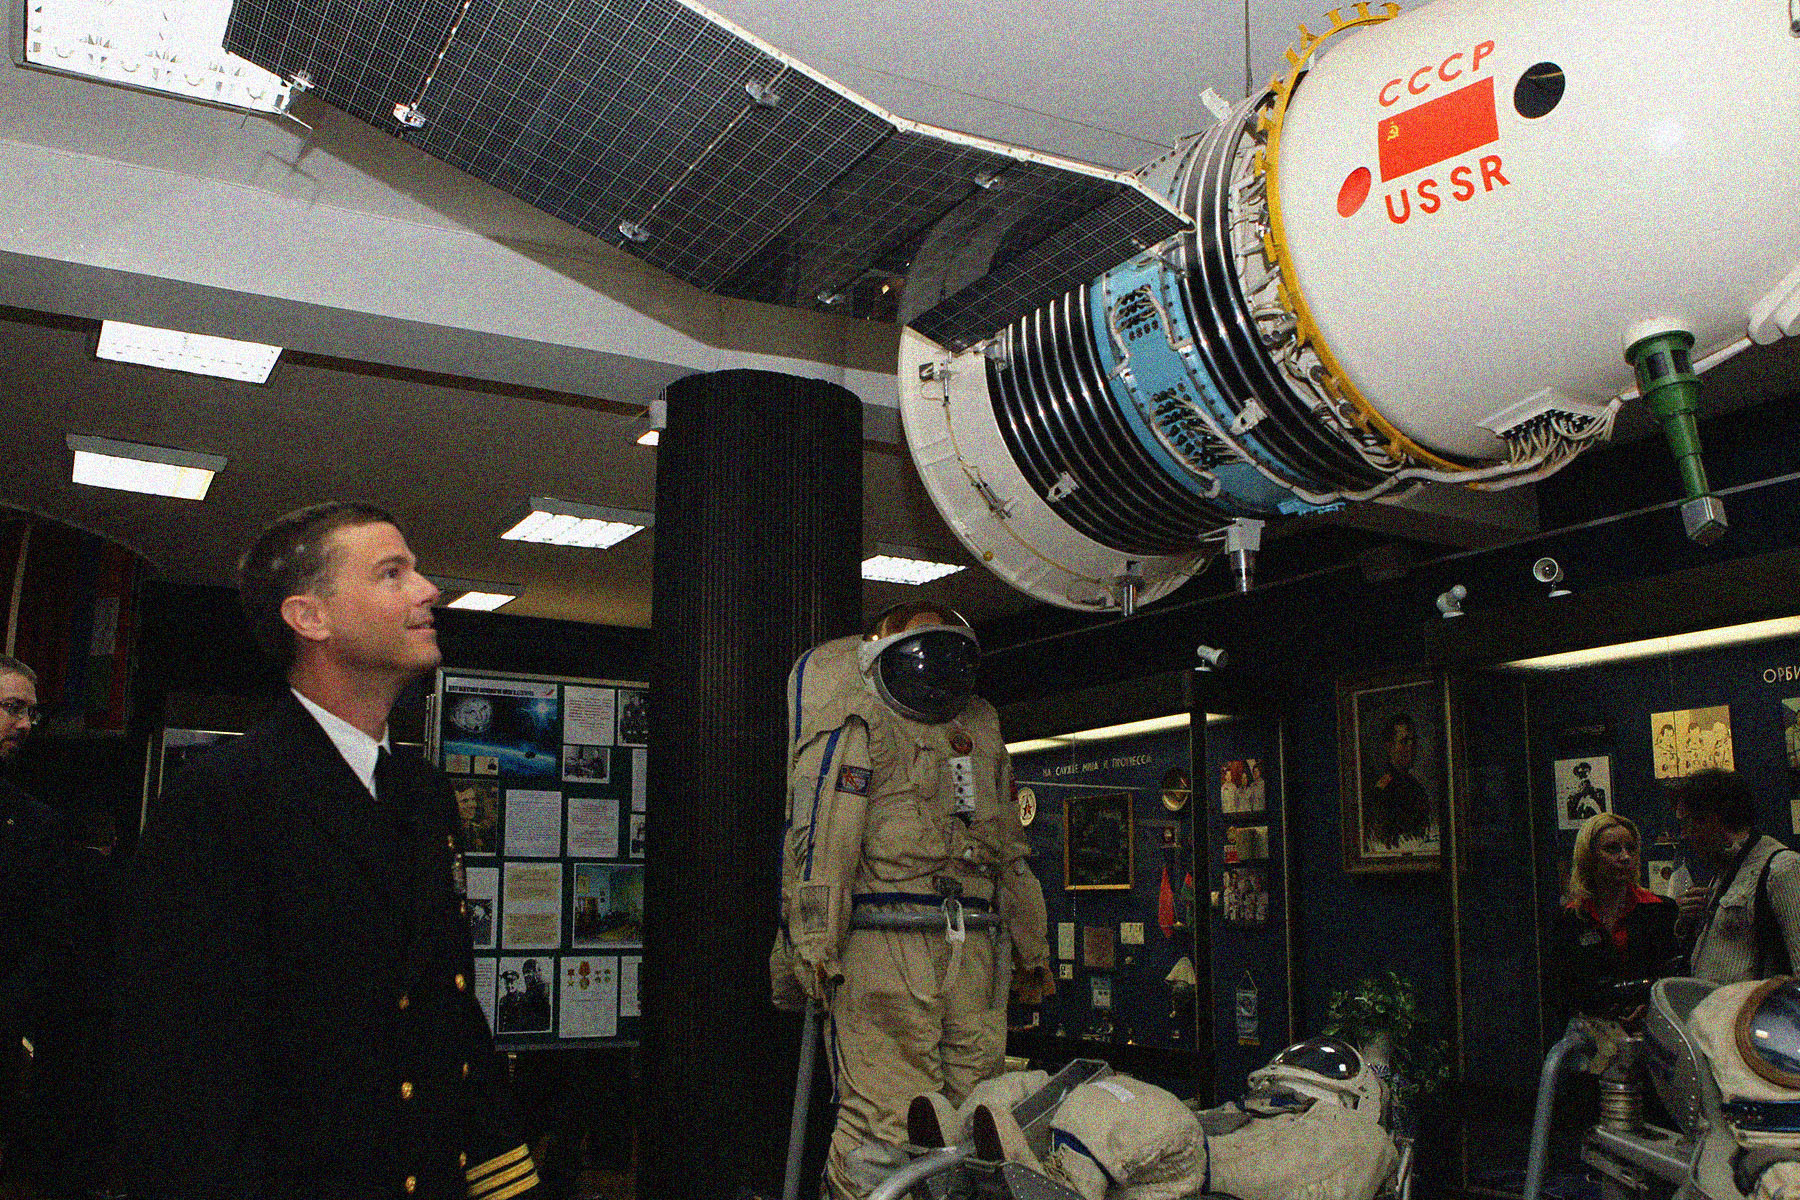
\includegraphics[width=0.32\textwidth]{codes/noise.jpg}}
    \subfigure[gaussian]{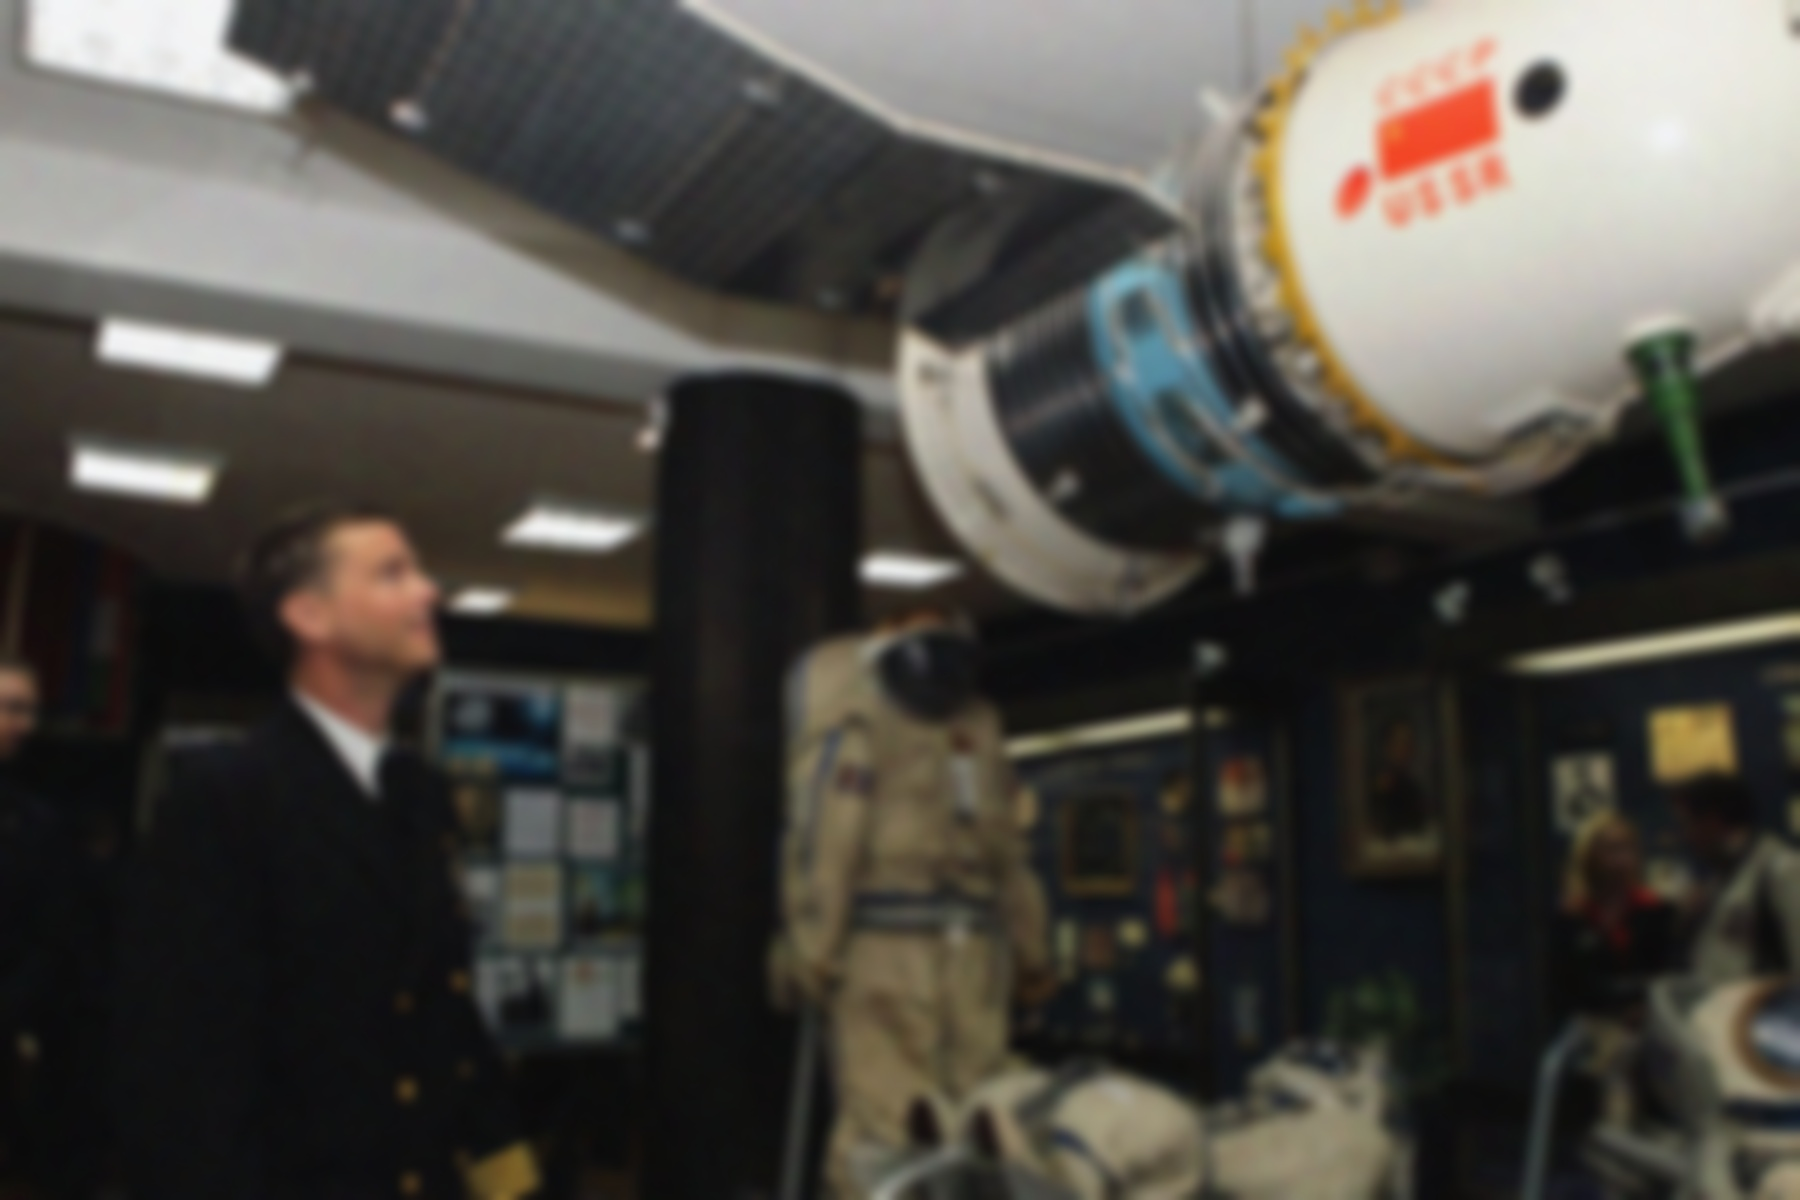
\includegraphics[width=0.32\textwidth]{img/noiseSuppressed.jpg}}
    \caption{(a) Original image of the Star City Museum\cite{NASA_on_The_Commons_14}(b) Noise added artificially (c) Blurred with Gaussian (k=27 $\sigma=7$)}
    \label{fig:noise}
\end{figure}\end{minipage}

Essentially, the three above filters are different mathematical functions applied both horizontally and vertically.\\
\begin{minipage}{\textwidth}\begin{figure}[H]
    \centering
    \subfigure[Average]{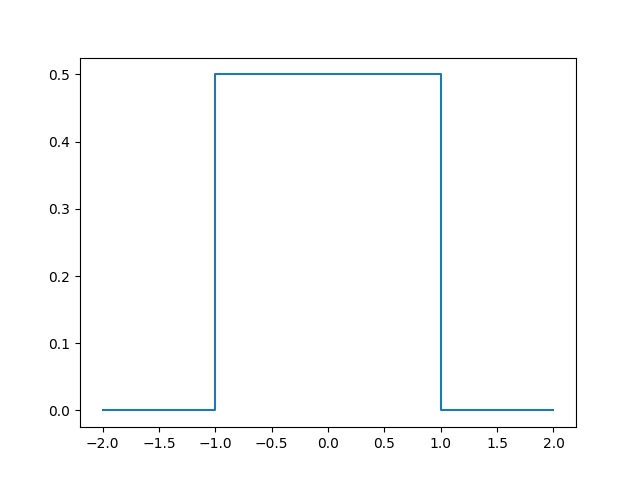
\includegraphics[width=0.29\textwidth]{img/box_graph.png}}
    \subfigure[Bartlett (Tent)]{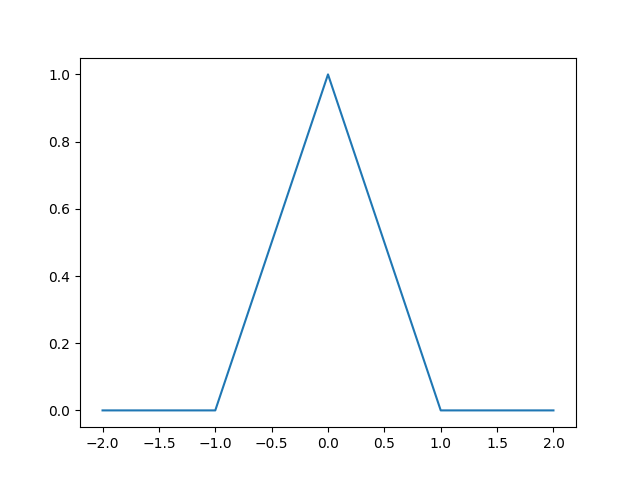
\includegraphics[width=0.29\textwidth]{img/tent_graph.png}}
    \subfigure[Gaussian]{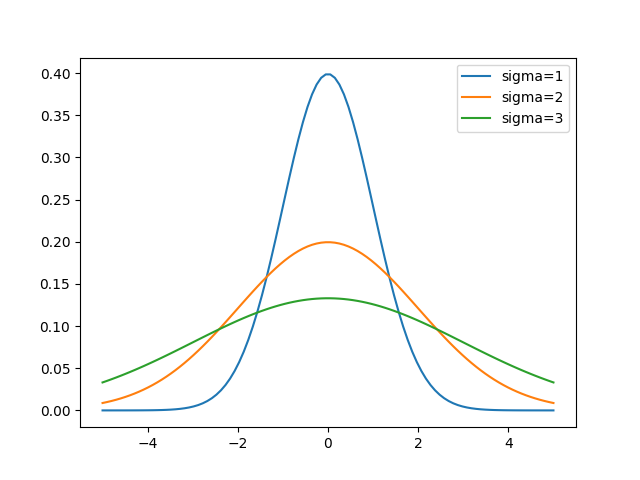
\includegraphics[width=0.29\textwidth]{img/gaussian_graph.png}}
    \caption{One dimensional graphs of the filters}
    \label{fig:graph}
\end{figure}\end{minipage}
As its name suggests, the Gaussian Filter is based on the Gaussian function (also commonly known as the normal function).
Two dimensionally, it can be expressed as \cite{MISRA2020289}
\[
    G_{2D}(x, y, \sigma) = \frac{1}{2\pi\sigma^2}e^{-\frac{x^2 + y^2}{2\sigma^2}}
\]
It can be seen from the graph that the lower the sigma value, the narrower the neighborhood becomes. 


\begin{minipage}{\textwidth}\begin{figure}[H]
    \centering
    \subfigure[Box $(k=133)$]{
\includegraphics[width=0.29\textwidth]{img/blurBox.png}}
    \subfigure[Gaussian $(k=233)$]{
\includegraphics[width=0.29\textwidth]{img/blurGaussian.png}}
    \caption{Comparison between gaussian and box blur}\label{fig:gauss_box}
\end{figure}\end{minipage}
From Figure \ref{fig:gauss_box}, using the gaussian blur, as opposed to
the box filter produces a more appealing image, as it preserves the shape of the image better as opposed to creating this `halo' effect
and producing a squashed rectangular shape in the center. One disadvantage to Gaussian however is, to produce an equally `blurred' image, a larger kernel is required for Gaussian, which can be argued to then be slower
than using the box filter\cite{Gonzalez_Woods_2018}.


These filters are mainly used to smoothen(blur) the image, where the low frequencies are let through as well as reducing the effect of the high frequencies (high frequencies and low frequencies both referring to
the brightness/darkness of each pixel). In practical applications, this is done to reduce high frequency noises.
A creative application to smoothing the images, is that the smoothen images can be used as a mask to sharpen the image by adding the difference between the original and blurred image.
This method is called \emph{unsharp masking}, aiming to enhance the difference between the shadows and higlights on an image\cite{Szeliski_2022}.
\[
  g_{sharp} = f + \gamma(f - h_{blur} \ast f)  
\]
\begin{minipage}{\textwidth}\begin{figure}[H]
    \centering
    \subfigure[original]{
\includegraphics[width=0.19\textwidth]{img/original_mask.jpg}}
    \subfigure[unsharp mask]{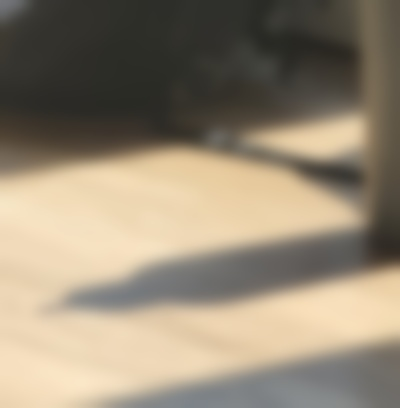
\includegraphics[width=0.19\textwidth]{img/unsharp_mask.jpg}}
    \subfigure[difference]{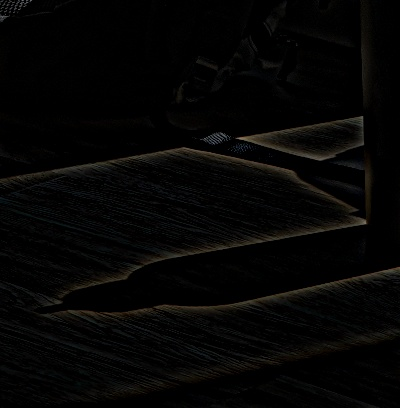
\includegraphics[width=0.19\textwidth]{img/difference_unsharp.jpg}}
    \subfigure[sharpened]{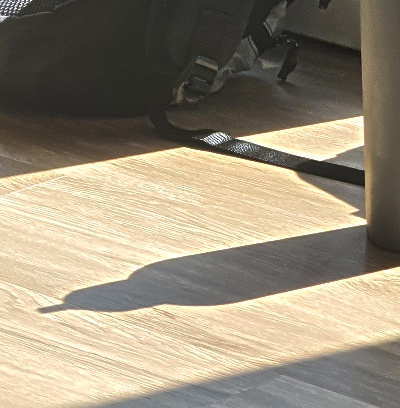
\includegraphics[width=0.19\textwidth]{img/sharpened.jpg}}
    \caption{Unsharp masking with Gaussian blur}\label{fig:unsharp_mask}
\end{figure}\end{minipage}
The result of the image traces a bright outline througout the image between the darker(shadow) and lighter part. It can also be seen, that
the difference between the blurred image and the original results in an approximate edge detection. A better way to extract edges by means of linear filtering is
by the use of the \emph{Sobel filter}. \cite{Szeliski_2022}

\subsection{Sobel Filter}
As per the example in the previous section, the horizontal Sobel operator is calculated by combining the \emph{horizontal central difference}
(which calculates the second horizontal derivative of the pixel and places it in the center itself) and a vertical linear tent filter to smooth the result. Respectively, it can also
be done for the vertical derivative.

The two sobel operator emphasizes the horizontal or vertical edges respectively, although as seen in the images, it can also highlight diagonal edges.\\
\begin{minipage}{\textwidth}\begin{figure}[H]
    \centering
    \subfigure[original]{\includegraphics*[width=0.29\textwidth]{codes/nasa.jpg}}
    \subfigure[horizontal]{\includegraphics[width=0.29\textwidth]{img/sobelHorizontal.png}}
    \subfigure[vertical]{\includegraphics[width=0.29\textwidth]{img/sobelVertical.png}}
    \caption{Vertical and Horizontal Sobel filtering\cite{NASA_on_The_Commons_2023}}\label{fig:sobel}
\end{figure}\end{minipage}

\subsection{Band-pass and steerable Filter}
In the above example, the sobel filter is calculated either for the horizontal or
vertical axis. Nevertheless, it is possible to calculate filters (including for sobel) for any angles in between using a specified 
\emph{directional derivative} $\nabla_{\boldsymbol{\hat{u}}} = \frac{\partial}{\partial\boldsymbol{\hat{u}}}$ 
and a \emph{unit direction} $\boldsymbol{\hat{u}} = (\cos \theta, \sin \theta)$\cite{Szeliski_2022}.
\[
    \boldsymbol{\hat{u}} \cdot \nabla (G \ast f) = \nabla_{\boldsymbol{\hat{u}}}(G \ast f) = (\nabla_{\boldsymbol{\hat{u}}}G) \ast  f
\]
Then it is also preferable to smooth it with the Gaussian filter.
\[
    G_{\boldsymbol{\hat{u}}} = u G_x + v G_y = u \frac{\partial G}{\partial x} + v \frac{\partial G}{\partial y} 
\]
This is called the \emph{directional} or \emph{oriented} filter.

A similar to operator to the sobel filter is called the \emph{Prewitt operator}, which instead of convolving it with a perpendicular tent filter,
it instead uses an average operator. Commonly however, the Sobel operator is preferred as it provides better performance\cite{NIXON2020141}. Through testing, the Sobel Operator seems
to be less selective than the Prewitt Operator, but one can argue that the Prewitt is then preferred as it is more accurate.

\begin{minipage}{\textwidth}\begin{figure}[H]
    \centering
    \subfigure[Pattern]{\includegraphics*[width=0.29\textwidth]{codes/pattern.png}}
    \subfigure[Sobel]{
\includegraphics[width=0.29\textwidth]{img/directionSobel.png}}
    \subfigure[Prewitt]{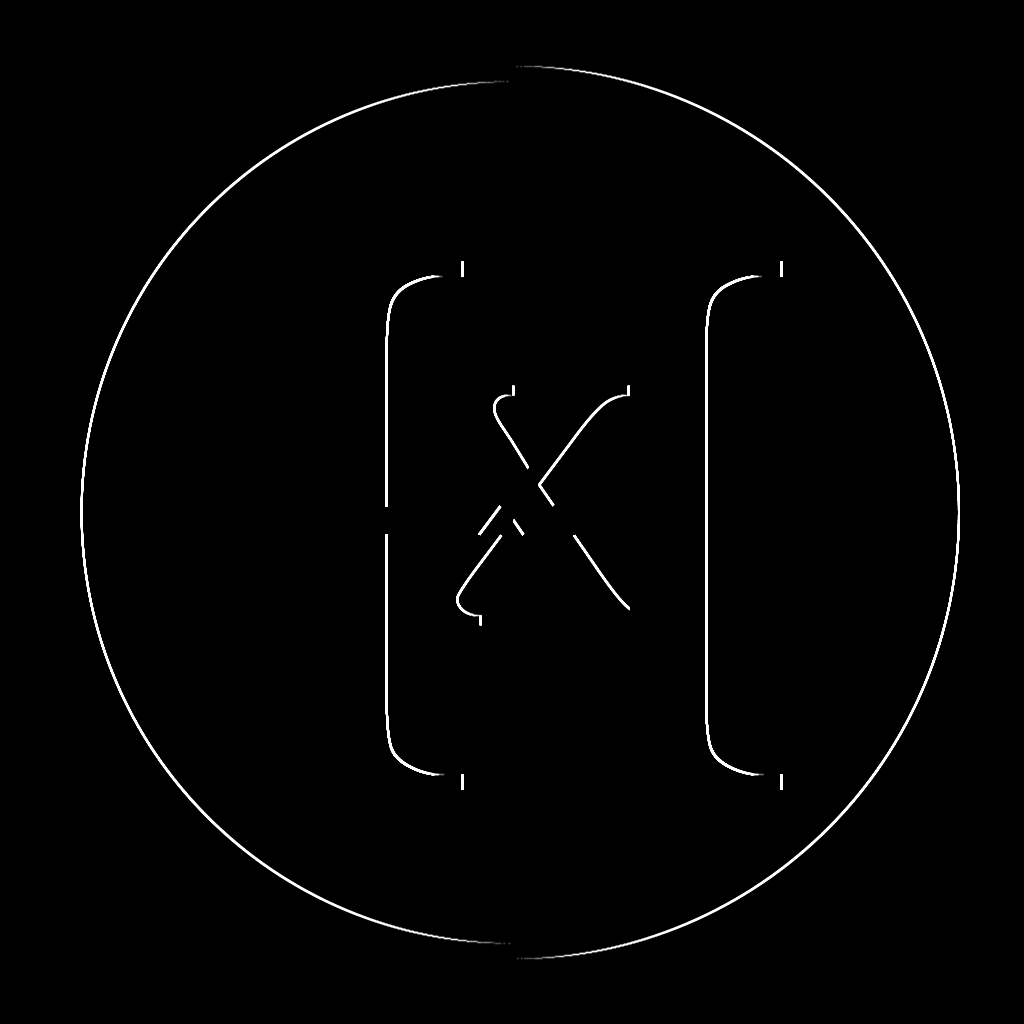
\includegraphics[width=0.29\textwidth]{img/directionScharr.png}}
    \caption{Vertical edge detection using Sobel and Prewitt on a test pattern}\label{fig:pattern}
\end{figure}\end{minipage}

As seen on Figure \ref{fig:pattern}, the Sobel filter tapers the edges at the top into a gradient, whereas the Prewitt marks it confidently without tapering. In practice however,
the minimal difference might not be worth the difference in the additional compute time \cite{NIXON2020141}.

\begin{minipage}{\textwidth}\begin{figure}[H]
    \centering
    \subfigure[]{
        {$\begin{bmatrix}
            -1 & 0 & 1 \\
            -2 & 0 & 2 \\
            -1 & 0 & 1
        \end{bmatrix}$}
    }
    \subfigure[]{
        {$\begin{bmatrix}
            1 & 0 & -1 \\
            1 & 0 & -1 \\
            1 & 0 & -1
        \end{bmatrix}$}
    }
    \subfigure[]{
        {$\begin{bmatrix}
            1 & 1 & 1 \\
            0 & 0 & 0 \\
            -1 & -1 & -1
        \end{bmatrix}$}
    }
    \caption{Sobel and Prewitt operator comparison (a) Horizontal Sobel operator; 
    (b) Horizontal Prewitt operator; (c) Vertical Prewitt operator}\label{fig:prewittSobel}
\end{figure}\end{minipage}


Another filter is called the \emph{Laplacian operator}, which is the second (undirected)derivative.\cite{Szeliski_2022}
\[
    \nabla^2 f = \frac{\partial^2 f}{\partial x^2} + \frac{\partial^2 f}{\partial y^2}
\]
and again, it can be smoothed with the Gaussian filter. It is equivalent to the \emph{Laplacian of Gaussian}(LoG) filter.
\[
    \nabla^2 G (x, y, \sigma) = (\frac{x^2 + y^2}{\sigma^4} - \frac{2}{\sigma^2}) G (x, y, \sigma)
\]
\begin{minipage}{\textwidth}\begin{figure}[H]
    \centering
    \subfigure[]{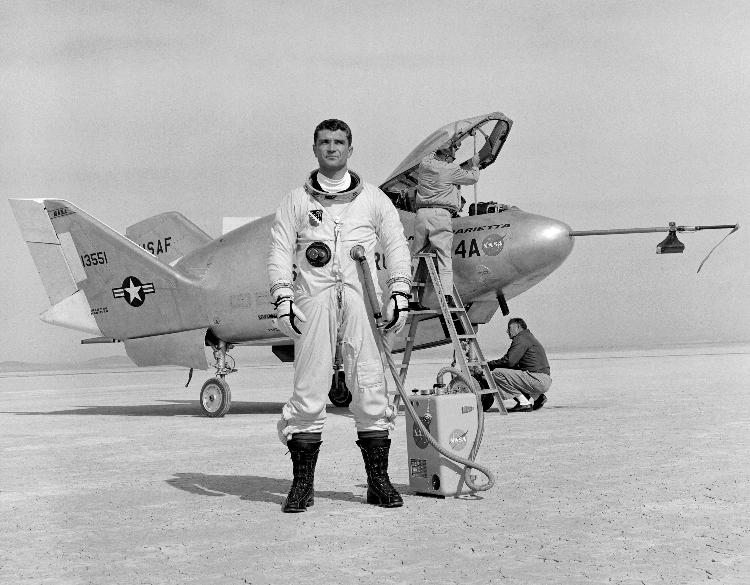
\includegraphics[width=0.29\textwidth]{img/laplacianOriginal.png}}
    \subfigure[]{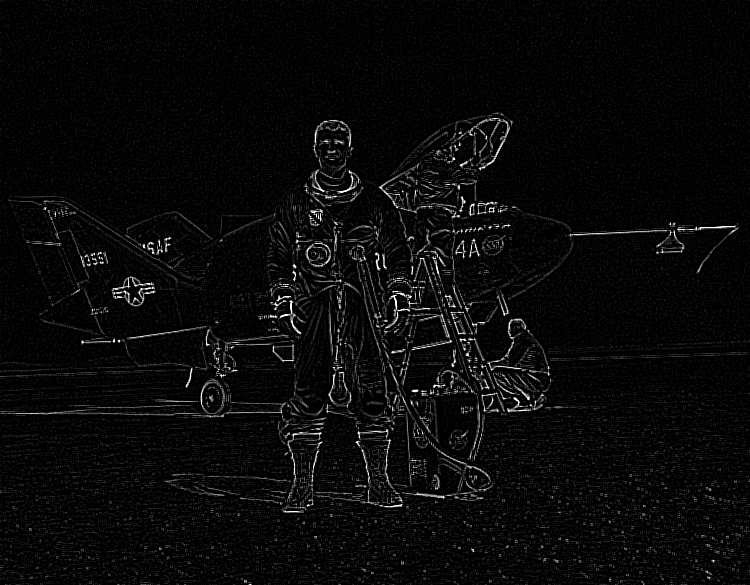
\includegraphics[width=0.29\textwidth]{img/laplacian.png}}
    \subfigure[]{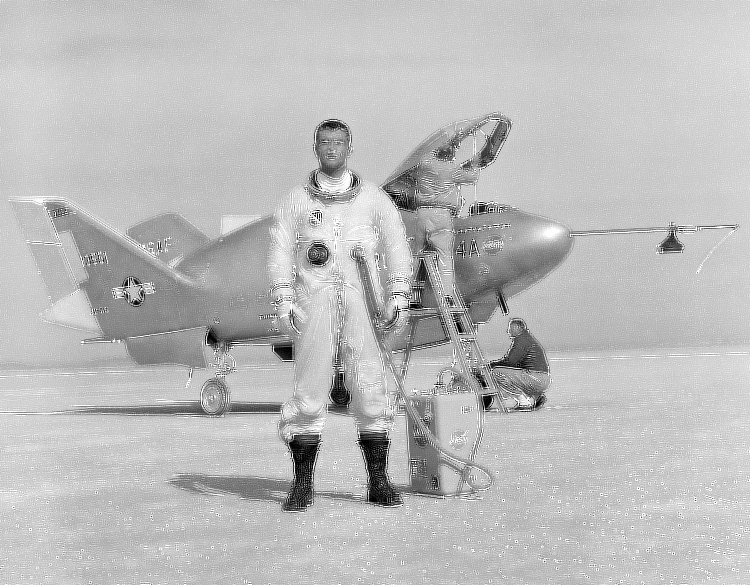
\includegraphics[width=0.29\textwidth]{img/laplacianAdded.png}}
    \caption{Laplacian Filtering (a) Original image of NASA pilot\cite{NASA_on_The_Commons_1970}; (b) Output of the laplacian filter with Gaussian blur (c) Combined image of the orientation map and original}
    \label{fig:padding_borders}
\end{figure}\end{minipage}

Since the laplacian filter does not rely on a specific direction, it can be seen at the above picture that the edges are agnostic to the direction and not biased to a certain angle. Bear in mind that smoothing the picture (in this case by means of the Gaussian filter)
is necessary as it subdues the noises from being detected as edges.

The aforementioned filters are more sophisticated as they require the second or first derivatives and they can filter both the low and high frequencies. 
These filters are called \emph{band-pass filters}.
Since the filters are based on the gradient fields, which are undirected, it can be `steered' by freely choosing a unit direction, hence the name
\emph{steerable} filter. The advantage of this is that multiple variations of directions can easily be calculated with minimal cost as the derivative must only be calculated once. In case of higher order derivatives,
the calculation must be done repeatedly with the same unit vector. This can although be calculated with a relatively small number of functions\cite{Szeliski_2022}. Consider the example below for the second-order derivatives,
which requires 3 basis functions. Although the basis filters are not in itself separable, it can be expressed as a linear combination of multiple separable filters.
\[
    G_{\boldsymbol{\hat{u}}\boldsymbol{\hat{u}}} = u^2 G_{xx} + 2uvG_{xy} + v^2 G_{yy} \text{with} \hspace*{0.5em}\boldsymbol{\hat{u}} = (u, v)
\]

With higher order steerable filters, it is possible to create filters that is more selective with the orientation (unlike in Figure \ref{fig:sobel}, where the lines placed at an angle of $45^\circ$ is highlighted). Alternatively,
it can also be possible to create filters that responds to more than one type of edge, whether bar edges (thin lines) or step edges (stark transitions between dark and light pixels), this however requires the \emph{Hilbert transform pairs}
\cite{Szeliski_2022}.

\begin{minipage}{\textwidth}\begin{figure}[H]
    \centering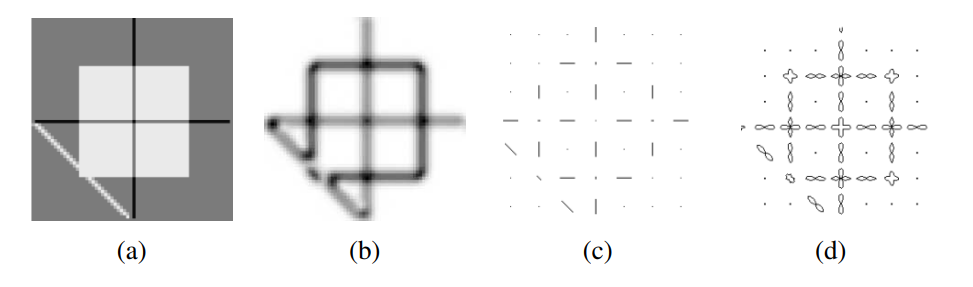
\includegraphics[width=0.60\textwidth]{img/higher.PNG}
    \caption{Fourth-order steerable filter (a) original test pattern (b) average oriented output (c) dominant orientation (d) oriented energy as a function of angle (polar plot)\cite{Szeliski_2022}}
\end{figure}\end{minipage}

Steerable filtering are most commonly used for edge detection, but another common use case is \emph{corner detection}. This requires multiple steerable operators in different directions as corners are defined as
points with a sharp change in direction (high curvature)\cite{NIXON2020141}. Feature description is also one application of steerable filter\cite{Szeliski_2022}.

With all the different kernels and each of their own applications, it is evident that even though linear filtering is fundamentally passing the weighted sum of a neighborhood, it can be a really powerful tool. Especially with today's hardware
linear filtering can be considered a quick and cost effective method for image processing.

\subsection{Summed area table (integral image)}
To calculate pixels in a neighborhood, some pixels needs to be accessed multiple times and as the kernel size increases, this problem also magnifies as well. To
better process the convolution of multiple box filters of different sizes and locations, preprocessing it can practically reduce the time complexity. 
This can be done with the
\emph{summed area table}, or the running sum of all the pixel values from the origin. It can be computed recursively through the raster-scan algorithm.
\[
    s(i, j) = s(i - 1, j) + s(i, j - 1) - s(i - 1,j - 1) + f(i, j)   
\]
This is also an example of recursive filtering, which takes a previous calculated value of a pixel and calculate it further for the next pixel. In this case, this can theoretically go on forever, but since no picture is infinite,
the edges can be calculated using the padding strategies in Section\ref{chap:padding}.

Since the calculations are based on previously calculated pixels, this attempts to reduce the amount of times a pixel is used for calculations, as it immediately takes the already calculated value
instead. The image $s(i, j)$, often called \emph{Integral image} can be computed using two additions per pixel. The summed area inside a chosen rectangl can be calculated by sampling 4 pixels from the summed area table.
\[
    S(i_0\hdots i_1, j_0\hdots j_1) = s(i_1, j_1) - s(i_1, j_0 - 1) - s(i_0 - 1, j_1) + s(i_0 - 1, j_0 - 1)
\]
 
\begin{minipage}{\textwidth}\begin{figure}[H]
    \centering
    \subfigure[Original image(S = 24)]{
        $\begin{tabular}{|c|c|c|c|c|}
            \hline 3 & 2 & 7 & 2 & 3 \\
            \hline 1 & \cellcolor{green!25}5 & \cellcolor{green!25}1 & \cellcolor{green!25}3 & 4 \\
            \hline 5 & \cellcolor{green!25}1 & \cellcolor{green!25}\textbf{3} & \cellcolor{green!25}5 & 1 \\
            \hline 4 & \cellcolor{green!25}3 & \cellcolor{green!25}2 & \cellcolor{green!25}1 & 6 \\
            \hline 2 & 4 & 1 & 4 & 8 \\
            \hline
        \end{tabular}$
    }
    \subfigure[Summed area table(S = 28)]{
        $\begin{tabular}{|c|c|c|c|c|}
            \hline 3 & 5 & 12 & 14 & 17 \\
            \hline 4 & \cellcolor{cyan!25}\textit{11} & \cellcolor{cyan!25}\textbf{19} & 24 & 31 \\
            \hline 9 & \cellcolor{cyan!25}\textbf{17} & \cellcolor{red!25}28 & 38 & 46    \\
            \hline 13 & 24 & 37 & 48 & 62 \\
            \hline 15 & 30 & 44 & 59 & 81 \\
            \hline
        \end{tabular}$
    }
    \subfigure[Computation of area sum (S = 24)]{
        $\begin{tabular}{|c|c|c|c|c|}
            \hline \cellcolor{blue!25}\textbf{3} & 5 & 12 & \cellcolor{blue!25}\textit{14} & 17 \\
            \hline 4 & \cellcolor{green!25}11 & \cellcolor{green!25}19 & \cellcolor{green!25}24 & 31 \\
            \hline 9 & \cellcolor{green!25}17 & \cellcolor{green!25}28 & \cellcolor{green!25}38 & 46 \\
            \hline \cellcolor{blue!25}\textit{13} & \cellcolor{green!25}24 & \cellcolor{green!25}37 & \cellcolor{blue!25}\textbf{48} & 62 \\
            \hline 15 & 30 & 44 & 59 & 81 \\
            \hline
        \end{tabular}$
    }
    \caption{Summed area tables\cite{Szeliski_2022}}
    \label{fig:graph}
\end{figure}\end{minipage}
The above table shows the relation of how the area is calculated. For summed area table, the red pixel is calculated by adding itself to the
two highlighted pixels in bold while subtracting the italicised symbol After the entire summed area table is calculated, it is now
cost effective to calculate the area sum as the sum of the top left and bottom right numbers only needs to be subtracted with the other diagonal (remember that
the starting indices requires it to go one pixel beyond the corresponding rectangle).

Although with this preprocessing it reduces the time complexity, the space complexity increases, since each pixel's range has now increased due to summing multiple pixel into a single pixel,
hence each of them now requires $\log M + \log N$ additional bits ($M$ and $N$ being the width and height)\cite{Szeliski_2022}.

A common use case for summed area table is for feature detections, computing simple multi-scale low-level features. In practice, it may be preferrable to instead use 
moving average filters, for example in computing the sum in the sum of squared differences stereo (SSD) and motion algorithms\cite{Szeliski_2022}.\footnotemark\footnotetext{Entire section of linear filtering is written by Jose}
 

% ========================================================================= ALEX

\section{Non-Linear Filters}
Non-linear filters serve as additional ways of filtering images. Linear filters can work exceptionally well for certain cases, however one will encounter scenarios where using Non-Linear filters will lead to a better result both visually (Image Processing) and performance-wise. One example noise removal, but more on that later. First of all it is important to look at what non-linear filters actually are.

\subsection{What are Non-Linear Filters?}
First and foremost, what are Non-Linear filters? As mentioned previously, linear filters are filters where the signal-response of two signals and the sum of the responses to the two signals individually are the same. Based on that one may probably guess that non-linear filters are filters where this criteria is not satisfied, and this is the case. This could mean that, in relation to the input data, the transformation could, for instance, be exponential as opposed to linear. This can lead to bigger difficulties concerning frequency response analysis,\cite[p.~132]{szeliski} shift-invariance, etc but also allow for greater flexibility. In certain scenarios this increased flexibility in transformations of the input signal (pixels) allows for greater accuracy, and as a result, better data.
\subsection{Some different types of Non-Linear filters}
\subsubsection{Median Filtering}
Consider a scenario with so-called salt and pepper noise, i.e. an image with noise consisting of sporadic black and white pixels. Were one to use for instance a Gaussian filter, one would quickly end up with a slightly blurred version of the original image. The noise would most likely still be there, simply in a slightly blurred format. Somewhat of a disappointment. There are however other methods of filtering, and for this scenario, a median filter would most likely do the trick.

\begin{figure}[H]
    \centering
    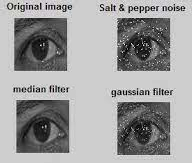
\includegraphics[width=0.5\linewidth]{medianfiltering.jpeg}
    \caption{The same image processed with a median filter and a Gaussian filter. Both filters remove salt and pepper noise (in varying degrees) and produce a result that more accurately corresponds with how the image should look without noise}
    \label{fig:enter-label} 
\end{figure}
Now we have seen an example median filtering, compared to Gaussian filtering, for a specific scenario, and what it does, it is time to dive into what a \textit{median filter actually is}. The algorithm works in this way: Given an input signal, in this case an image, it goes through every single pixel of the image, and replaces the value with the median value of the adjacent pixels. One can also let it go through the image whilst checking adjacent pixels in a 3px, 10px, or generally X-pixel radius around the current one, and replace it with the median of the pixels inside this X-pixel radius. The "X-pixel radius" is called a kernel. Increasing the kernel-size of the filter might lead to a "smeared" and somewhat blurry look in many scenarios.
\begin{figure}{h}
    \centering
    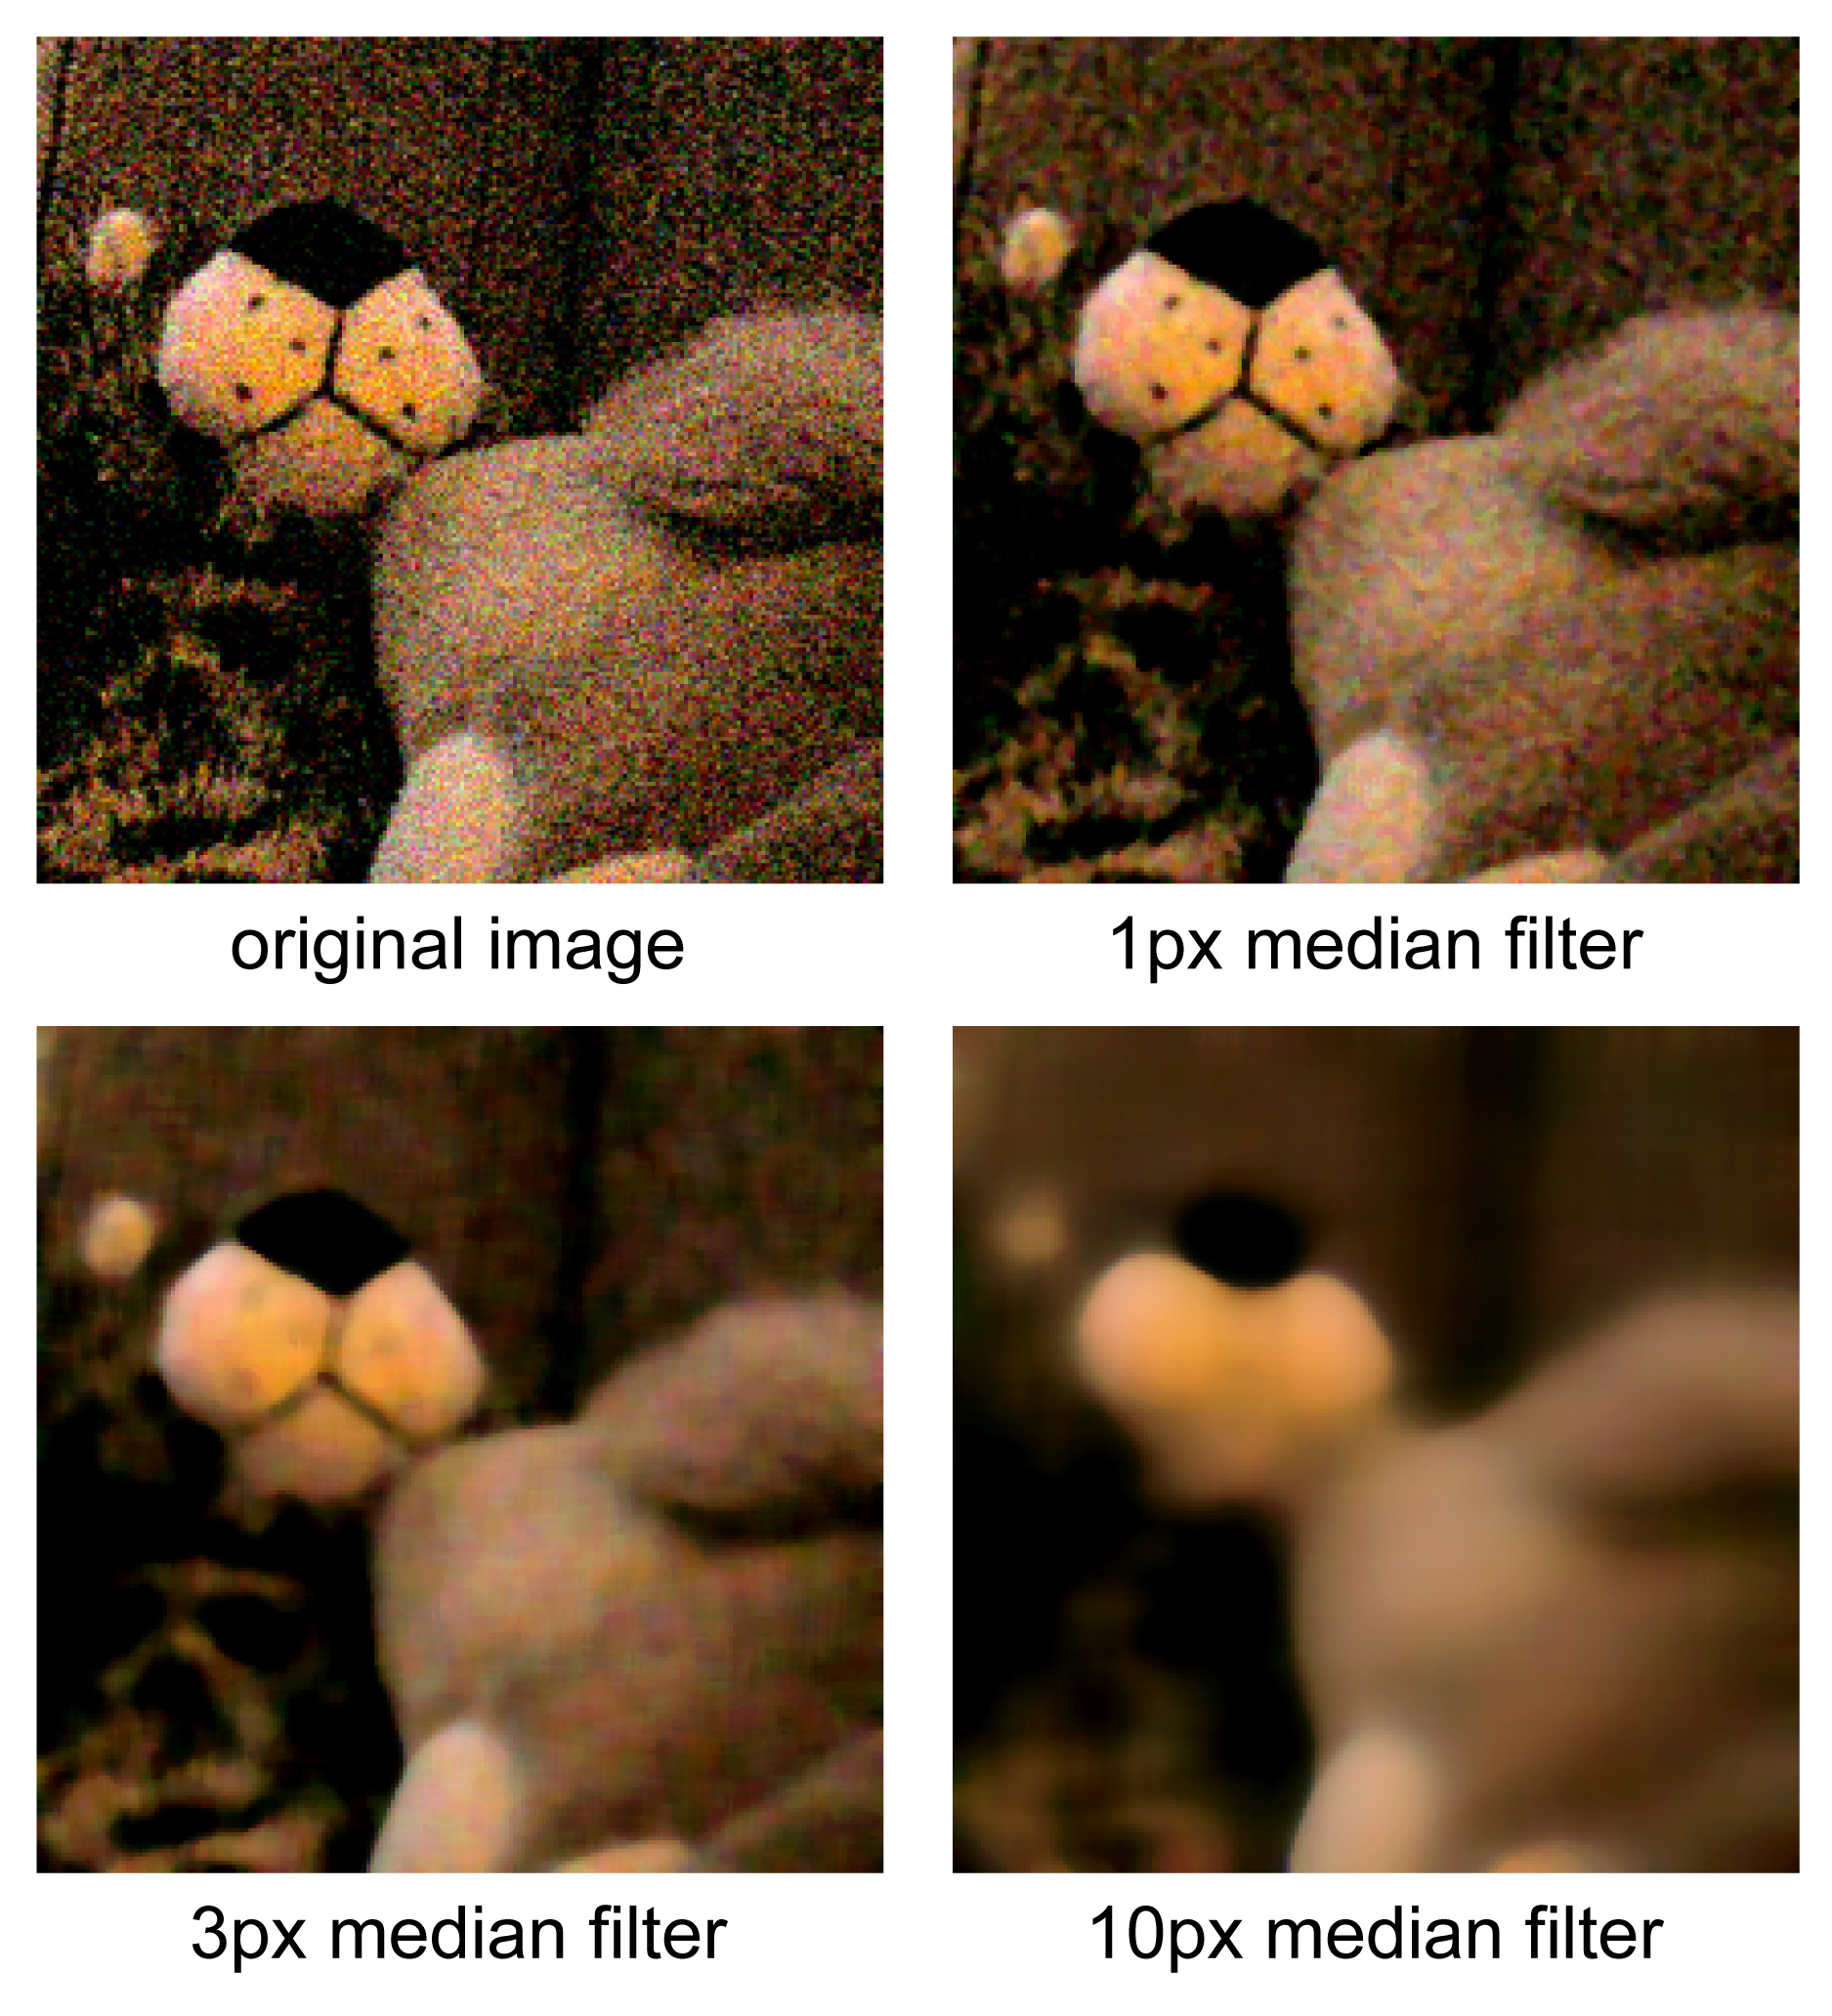
\includegraphics[width=1\linewidth]{median_example.jpg}
    \caption{Processing the image with a bigger kernel radius leads to less "crispness"}
    \label{fig:enter-label}
\end{figure}
\begin{figure}{h}
    \centering
    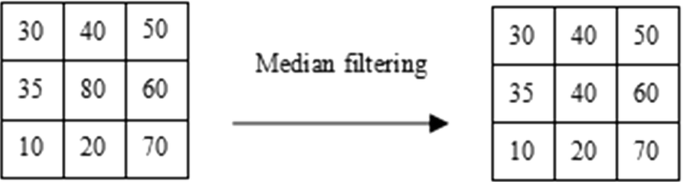
\includegraphics[width=1\linewidth]{medianfiltering.PNG}
    \caption{lllustration of how the mean filter algorithm works. The central pixel's value is changed from 80 to 40. 40 is the median of all the values within a 1px radius of the central pixel.}
    \label{fig:enter-label}
\end{figure}
However, even though median filters work relatively well for this specific scenario, the cure for cancer is yet to be found. There are (several) scenarios in which median filters might produce sub-optimal results.

\subsubsection{Bilateral Filtering}
Another type of Non-Linear filter is the bilateral filter. In order to properly understand the bilateral filter, it is first important to understand a few other principles.

It would, at this point, be prudent to mention a certain property of filters that can be very much sought after, namely, \textit{edge-preservation}. When filtering away noise one often runs the risk of losing the clarity of the edges in the image. Given an image with a coin, and some noise, one might filter away the noise with a filter, perhaps a Gaussian would work here. After applying the filter, the noise might have been cleared away, but one will often recognize a certain "smudgyness" by the edges. The, perhaps, once sharp clear edges where the coins meet the background have seemingly melted more into their surroundings. Somewhat problematic. Applying an even stronger filter might remove the clear edge of the coins completely, making the coins look more like the sun in the middle of day than the coins they supposedly are.
\begin{figure}[H]
    \centering
    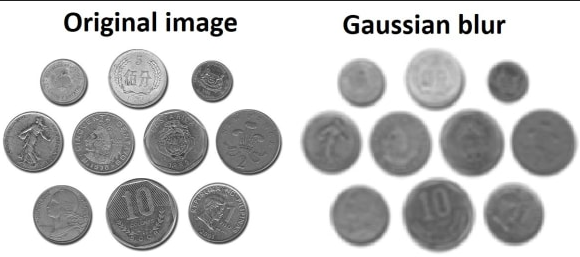
\includegraphics[width=1\linewidth]{coins.PNG}
    \caption{Applying a Gaussian-filter has made the edges of the coins less pronounced. This goes for the background-coin-edge, and also the edges of the coin details such as numbers and figures}
    \label{fig:enter-label}
\end{figure}

Another important filtering method to recognize, at this point, is weighted kernel filtering. Weighted kernel filtering is an extension of the median filter. It works by \textit{weighting} pixels based on their distance from the middle. I.e. the further the pixel is from the center, the smaller the effect of it, but importantly, it still has an influence! Typically, the weighted median is calculated as follows:
\begin{figure}[H]
    \centering
    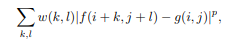
\includegraphics[width=0.5\linewidth]{weightedmedian.png}
\end{figure}
Now to bilateral filters themselves. 
\begin{figure}[H]
    \centering
    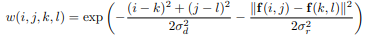
\includegraphics[width=0.75\linewidth]{bilateral.png}
\end{figure}
\textit{or the bilateral weight function} where i, j, k and l the weighting coefficients are dependent on the current kernel.
The base principle of bilateral filtering is applying the concept of weighted median filtering, yet with a tweak. The bilateral filter rejects values that are too much of an outlier for the current kernel, hence, often preserving edges better than the previously mentioned filters. Since a median filter uses all pixel-values in the kernel when processing an image, it may very well lead to blurred edges. Imagine, for instance, the aforementioned example with the coins (Figure 3.4). When the median filter does it's magic on the edges, for instance where the coin meets the background, it will use the values of the white background, and mix it into the values of the darker coins edges. Ergo, the edge of the darker coin will turn into a lighter colour because of the influence of the background. Apply the median filter several more times, and this will happen again and again and again, quickly leading to an unrecognizable blur, rather than a crisp clear image of coins with the noise removed (Note: This will most likely happen regardless of filter if one applies it an excessive amount of times, but the amount of times one must apply the filter for the image to become unrecognizably blurry or smudge-like is different).

Let's consider filtering the same image with a bilateral filter. When the bilateral filter considers pixels along the edge of the coins it will not consider outliers, hence, it will not consider the pixels of the strong white background, rather focusing on the pixels of the coin itself, as they are more similar to the relevant pixel. That is not to say that applying the bilateral filter an exorbitant amount of times won't lead to the edges eventually blending into their surroundings, but the bilateral filter does, for most intents and purposes, preserve edges.


\subsubsection{Minimum- and Maximum Filtering}
Two more types of non-linear filters are minimum- and maximum filters. These two filters are often also called dilation and erosion filters, respectively. They are classified amongst the so called morphological filters. In many ways, the minimum and maximum filters are two sides of the same coin, they are very similar in all but one point. As the minimum filter moves along the image, processing as it should, it simply chooses the smallest value inside the current kernel and applies this value to the relevant pixel. Maximum filters work very similarly, but, as one might guess, they instead pick the largest value and assigns that to the relevant pixel. Given the two filters other names, dilation and erosion, it might not be too much of a leap to assume what an image processed by these filters would look like relative to the original. Minimum filters, or dilation filters, simply dilate the darker areas of images (since darker values tend to be assigned lower numbers). Effective if one wishes to thicken the borders of a dark-coloured letter on a light background in an image. Contrarily, the maximum filter, or erosion filter, will erode darker pixels from images. If a black pixel is surrounded by only white pixels, it will be gone after an erosion filter has been applied.
Lastly on minimum and maximum filters, a bit about binary images. What are binary images? They are in fact part of what led to the creation of morphological filters such as the here discussed minimum and maximum ones. As one might deduce from the name "binary images"  they operate with \textit{only} binary values. In other terms, each pixel can only have one of two values, black and white.
\begin{figure}[H]
    \centering
    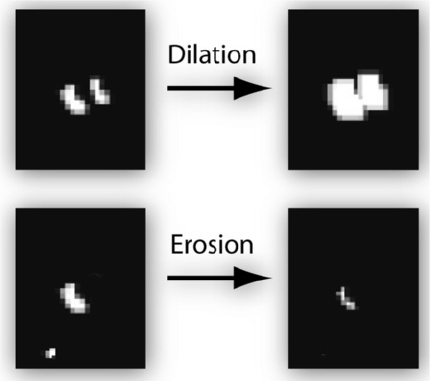
\includegraphics[width=1\linewidth]{minmax1.png}
    \caption{Illustrates the usage of minimum and maximum filters on a grayscale image. Using the minimum filter expands the area of the figure, whereas applying a maximum filter reduces it's size}
\end{figure}

\begin{figure}[H]
    \centering
    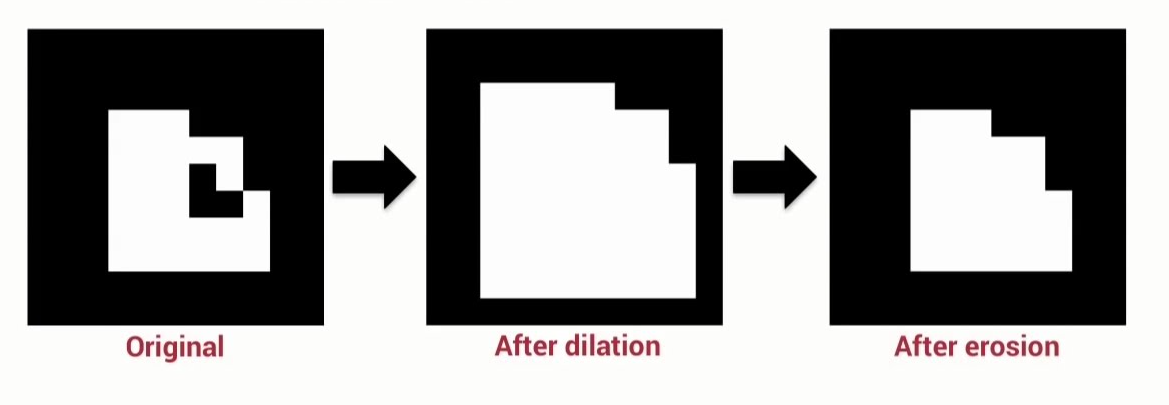
\includegraphics[width=1\linewidth]{minmax2.PNG}
    \caption{Illustration of three binary images. Using a minimum filter succeeded by a maximum filter fills the gaps in the figure and then decreases it's size (closing)}
    \label{fig:enter-label}
\end{figure}

\begin{itemize}
    \item Majority
    \item Opening
    \item Closing
\end{itemize}
Majority filters are a type of morphological filter that can help reduce noise, as well as make an image appear smoother. Their application is very similar to the application of a median filter

Opening and closing filters are closely related; they are both two step operations.
An opening filter starts by applying a maximum filter, then a minimum filter. This can help filter away unwanted noise, or other small objects, whilst still keeping the larger objects as they were. A closing filter on the other hand starts by applying a minimum filter, followed by a maximum filter. This help fill up gaps in figures whilst leaving the rest of the shape unaltered. Applying the closing filter several times (iteratively) will help fill up even bigger gaps in figures (gap will progressively shrink in size for every iteration).

\subsection{Guided Filter}


\subsection{Further Non-Linear filter related techniques}
\subsubsection{Mean Shift}
The mean shift algorithm is often referred to as a "hill climbing algorithm". Given for instance a scatter plot, or such, the mean shift algorithm will locate the area of the plot where the data-point density is at it's highest, metaphorically speaking, a hill (densest data cluster). Roughly, the algorithm will move (shift) from data point to data point based on the regional mean (mean of current cluster). What is considered in calculating the mean may vary from implementation to implementation. Some times calculating a weighted mean may yield more accurate results, depending on what one is searching for.
How can one apply this concept in image processing? Mostly in image segmentation. As mean shift is quite prolific at finding and recognizing clusters, it is also quite good at recognizing "clusters" in images, i.e. different parts of an image. Segmenting an image, categorizing different parts of it, can allow you to perhaps apply different filtering algorithms for different areas of the image, maybe help with edge detection, and in general help preserve the intended look and data of the image. Furthermore it has applications in for instance computer vision and pattern recognition. Important (sub-)fields of image processing.
\begin{figure}[H]
    \centering
    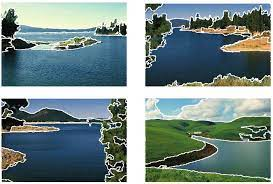
\includegraphics[width=1\linewidth]{meanshift.jpeg}
    \caption{Four different images, all segmented by a mean shift algorithm. The segmentation enables one to analyze different areas in different ways. Maybe one would rather filter noise away from water-areas or different coloured areas with different filtering techniques}
    \label{fig:enter-label}
\end{figure}
\begin{figure}[H]
    \centering
    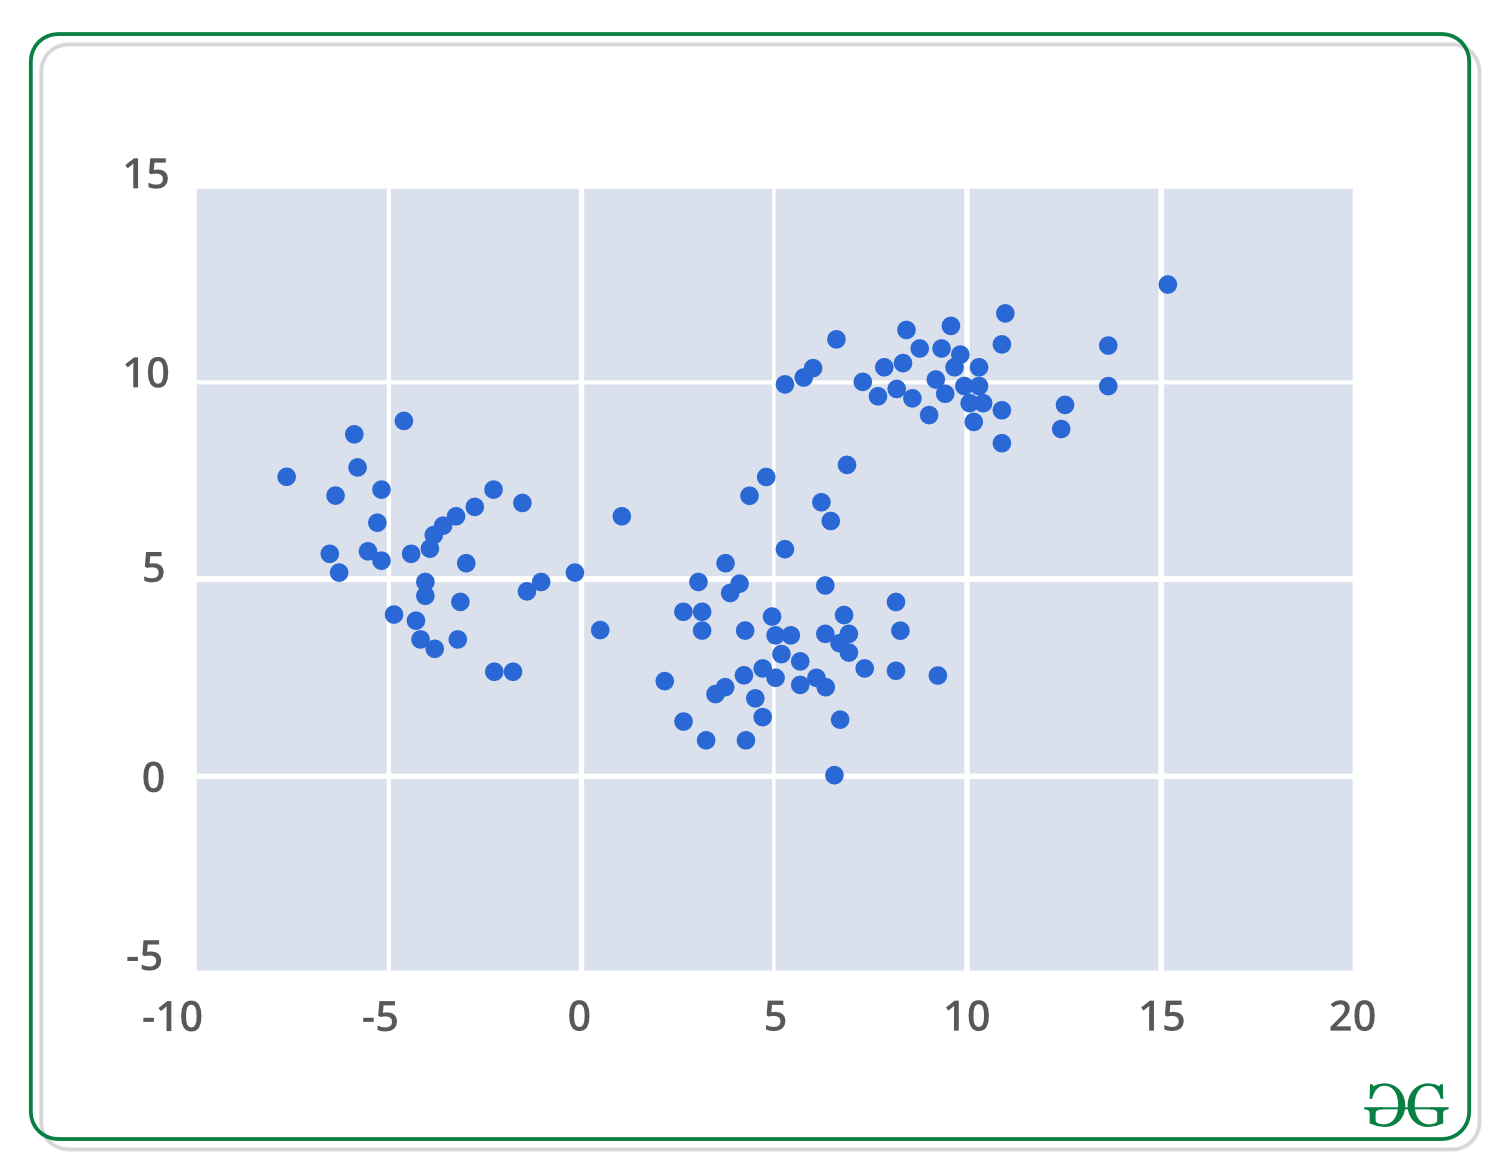
\includegraphics[width=1\linewidth]{scattergraph.png}
    \caption{A typical graph for which the mean shift algorithm could be applied. The clusters can be viewed as hills. Increased data point density would imply a "steeper hill". One can roughly recognize the outline of three main clusters here}
    \label{fig:enter-label}
\end{figure}

\subsubsection{Cellular Automata}
Cellular automata is something one probably has heard about in other contexts than image processing. Tracing it roots back to the late 40s, as the brainchild of the two late great scientists Stanislaw Ulam, and of course, the father of computer science himself Neumann Janos, commonly known as John von Neumann. Von Neumann was working on self-replicating-systems when he, with some help from Ulam, came up with his Cellular Automaton. Proving that his self-replicating automaton would work. But how can one apply this seemingly unrelated part of computer science to image processing?  First of all, let's assess how cellular automata work.

In essence, cellular automata are grids of cells, each containing what can be considered a finite state machine. They can be very useful in the analysis of many different systems, as well as in the fields of physics and biology. A famous example/application of cellular automata is Conway's game of life\cite{gardnermathematical}.
Now how specifically does one apply a cellular automaton to image processing?  As of now one of the most major application areas is noise removal in binary images. \cite{inproceedings} As demonstrated by Rosin and Sun\cite{rosin} it can also be used for edge detection, which, as previously mentioned, is an \textit{essential} part of image processing.
\begin{figure}{H}
    \centering
    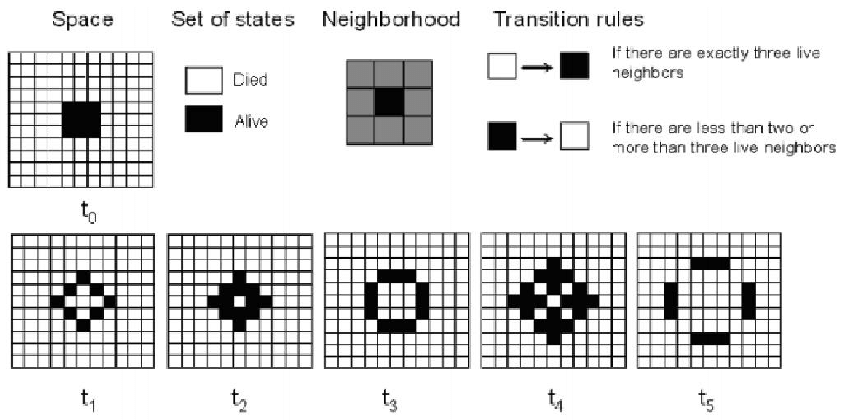
\includegraphics[width=1\linewidth]{gameoflife.png}
    \caption{An illustration of Conway's game of life. An important milestone in the study of Cellular Automata, and also a good example of what Cellular Automata can look like}
    \label{fig:enter-label}
\end{figure}
\subsection{Anisotropic Diffusion}
As discussed, there are several scenarios in which non-linear filters can help improve the clarity of images, but sometimes one may actually wish to blur certain areas of an image. Say, for instance, one wishes to recognize the outline of a person, an animal, a car, or similar in an image. Using edge-detection one might well find the edges accurately, but what when the edge-detection algorithm also detects features of the figures as edges, and not only the outline? This is where (anisotropic) diffusion can come into play. Diffusion in general will "smudge out" the image, letting edges and borders flow into one another creating an image where shapes may be hard to distinguish from one another. This is useful, as this is, in a sense, what we wish to do with the "inner details" of the figure we are trying to find the outline of. Still, there is somewhat of a problem remaining, the fact that only diffusing the image will lead to \textit{all} the edges and borders being hard to detect. Where anisotropic diffusion veers of from standard diffusion is by preserving the strongest edges or borders, the outlines. By controlling what is diffused and not, we diffuse only the contents inside the borders, hence making the most prominent edges all the more prominent relative to the rest of the image. This will allow us to figure out the outline of a figure more accurately, as the outline tends to be the most prominent border.
\begin{figure}[H]
    \centering
    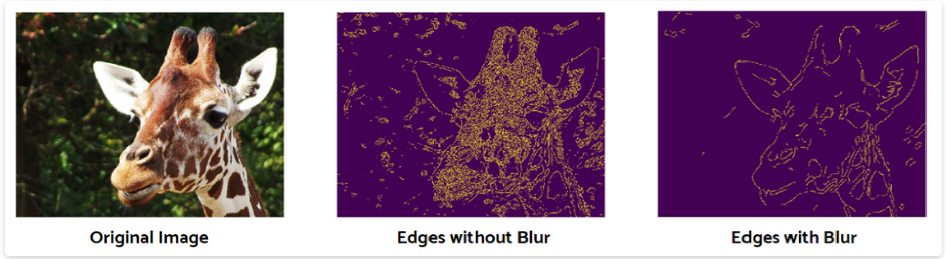
\includegraphics[width=1\linewidth]{edgedetection.png}
    \caption{Filtering can be a double edged-sword. Depending on what data one is searching for, one may not need to preserve every single edge in an image. For this scenario, if one is trying to recognize a clear outline of the giraffe, it is easier to find in a blurred version of the image}
    \label{fig:enter-label}
\end{figure}

\subsection{Typical applications of Non-Linear filters}
The subject of where one can apply Non-Linear filters has already been touched upon. Likely, the most prominent application area of non-linear filters in image processing is in noise filtering. Filtering away noise can be invaluable for increasing the clarity of a given image. A further application of non-linear filters is edge detection. Edge detection can be of vital importance (quite literally) in image processing, especially when applied in the context of computer vision, and for instance, autonomous cars. Non-Linear filters may also help in image enhancement and restoration, mostly through aforementioned applications such as noise-removal, pattern recognition (edge detection/segementation) and further techniques such as increasing contrast. Image restoration and enhancement can even be used to increase the resolution (upscaling) of images and videos, allowing old films to be re-released in higher resolutions. From the old graininess of VHS to HD and full HD all the way to UHD and 4k/8k resolutions. This process is of course not magic though, and it cannot create something that does not exist, hence it also cannot recover completely lost information\cite{sharmila}\footnotemark\footnotetext{Entire Section of Non-linear Filters written by Alex}
\begin{figure}[H]
    \centering
    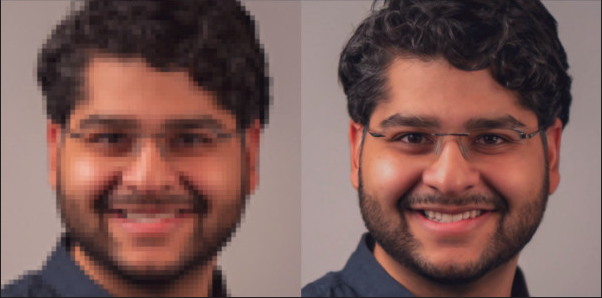
\includegraphics[width=1\linewidth]{upscaling.PNG}
    \caption{Non-Linear filtering can be a vital component in image enhancement and upscaling. In this photo the image has been upscaled from 64x64 to an impressive 1024x1024}
    \label{fig:enter-label}
\end{figure}

\section{Conclusion}
Now that we have discussed some different image processing algorithms, specifically several linear and non-linear filtering ones it is time to assess their use cases, and to compare them. A first obvious question that may arise is whether any specific type of filtering is simply objectively better. As with many situations in life, and different fields of computer science, this is hard to find. Just as it may be hard to determine a specific sorting algorithm as objectively the best in any given scenario, it is equally hard to determine an objectively best filtering algorithm. In some programs or prototypes it may be prudent to apply a simple filtering algorithm as nothing too extensive is needed. For ease of use and understanding, many linear filters may well hold the edge over most non-linear filters. Many non-linear filters can seem less intuitive, and hence be harder to understand and implement, possibly being overly complex for certain scenarios. It is also important to note that in most use cases, be that in pure image processing, signal processing or computer vision, many filters are used in combination to achieve optimal results. Applying specific filtering techniques for specific scenarios and then weaving all the data they produce together may well produce far more accurate data than taking a "one-size fits all" approach to filters.

Filtering can be an incredibly helpful tool in processing images. Removing noise from images, increasing clarity, detecting edges and such have applications in the closely related field of computer vision as well, but none of this comes without it's drawbacks. As we have seen, applying a wrong filter can easily lead to a decrease in clarity of images, perhaps only succeeding in making an image more blurry. Moreover, even if applying "the optimal" filtering algorithm it by no stretch of the imagination guarantees a completely noise and error free result. Filtering is not magic, certain images may be past a point in which it physically cannot get any clearer. This also leads into another issue, namely over-processing. Passing a signal or an image through a filter one time (or more) too many can lead to results which no longer resemble the original, what it was supposed too look like, or lead to unnatural results. In these cases, one may very well consider whether the application of a filter actually helped. If one in certain scenarios realizes that the answer for this case was actually no, one may already have spent far too many resources and hours on something that ended up being producing nothing practical. Resource management is very often of the essence.
\begin{figure}[H]
    \centering
    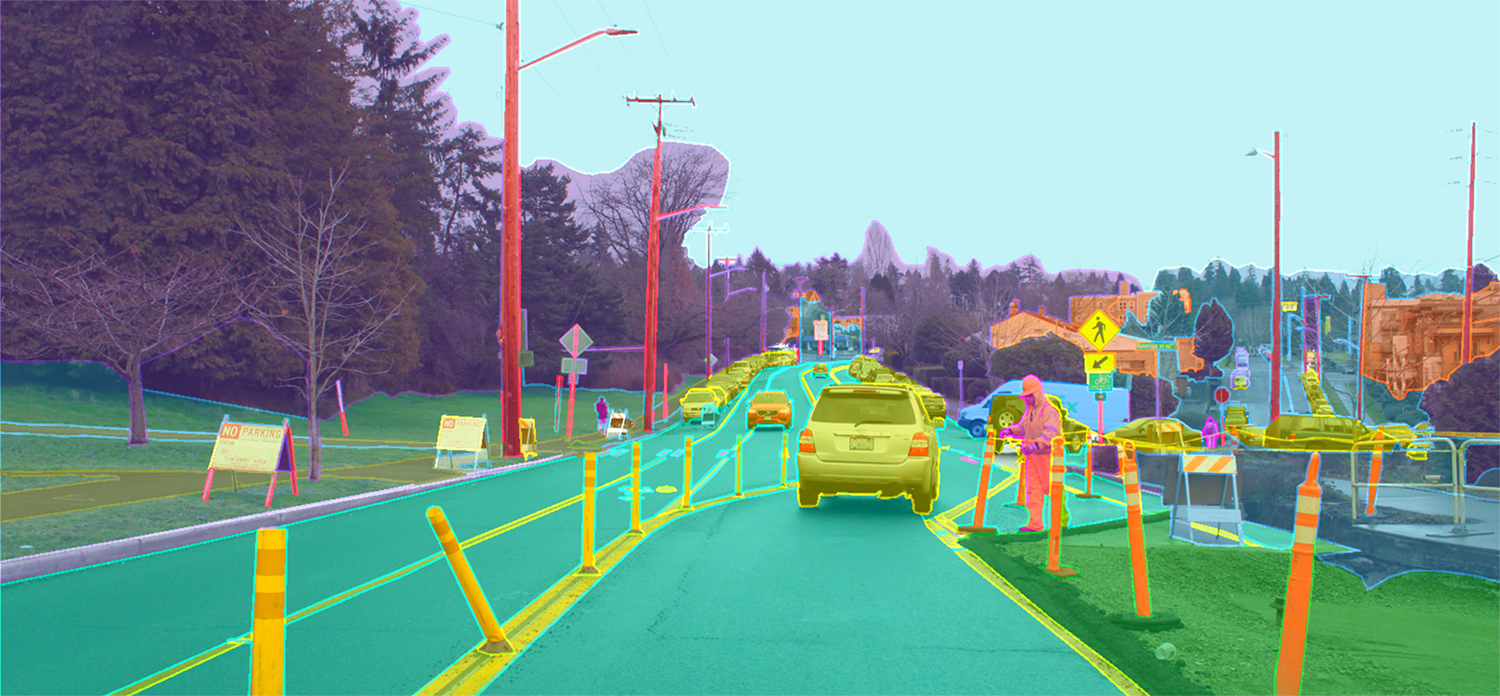
\includegraphics[width=1\linewidth]{csvision.jpg}
    \caption{Filtering an image to increase the clarity of it for computer vision algorithms is essential. Image segmentation algorithms like mean-shift filters allows the car to recognize different objects. If parts of an image are not clearly segmented, this can lead to misinterpretations. Maybe the self-driving car will assume something to wrongly be a part of something else}
    \label{fig:enter-label}
\end{figure}
Even with all the potential drawbacks that filtering can bring, the pros most likely heavily outweigh the cons. As technology advances, new techniques and new equipment will lead to even more advanced image processing. With the advent of AI, many of it's techniques may be appended to already existing techniques, or spawn new ones entirely. This will all surely lead to even more advanced filtering techniques, and with the blistering increase of data (big data) out there, there is no lack in training data for all AI/ML/Neural Network's needs. This will probably be the most major source of improvement for future filtering techniques. Another important area of improvement is efficiency. Increased hardware performance will lead to faster filtering algorithms working even more efficiently. Further research, and development of the algorithms will also lead to a better (lower) time-complexity, hence increasing the filtering algorithms efficiency further. This is of the utmost importance in, for instance, computer vision for autonomous cars. Faster processing and filtering of the image data a self-driving car collects can be the difference between life and death, and can drastically improve the safety of these self-driving cars.\footnotemark\footnotetext{Written by Alex}

% =========================================================================
\bibliographystyle{alpha}
\bibliography{abbrev, Draft}
\end{document}
